% CS5903 Distributed AI Training -- Final Project Report, Project 24, Group 2
% Build: pdflatex Project_Report.tex (twice). Figures are read from figures/ (copied from
% evaluation/report_pack/figures/). Fill the \TOFILL items before submission.
% Layout: "Notebook" theme. Engineering-notebook feel: mono headings, highlighter marks, graph paper. Text unchanged.
\documentclass[10pt,a4paper]{article}

% ---------- Page and fonts ----------
\usepackage[a4paper,margin=2cm,top=2.3cm,bottom=2.2cm]{geometry}
\usepackage[T1]{fontenc}
\usepackage[utf8]{inputenc}
\usepackage{utopia}
\usepackage[scaled=0.92]{helvet}
\usepackage{courier}
\usepackage{microtype}
\linespread{1.05}
\newcommand{\headfont}{\ttfamily}

% ---------- Colours ----------
\usepackage[table]{xcolor}
\definecolor{ink}{HTML}{1C2541}          % navy ink
\definecolor{accent}{HTML}{2B59C3}       % pen blue
\definecolor{hl}{HTML}{FFF176}           % highlighter yellow
\definecolor{pinkhl}{HTML}{FFC1D6}
\definecolor{skyhl}{HTML}{C8E6FF}
\definecolor{pen}{HTML}{E0457B}
\definecolor{muted}{HTML}{6B7794}
\definecolor{gridcol}{HTML}{DCE6F7}
\definecolor{rowgray}{HTML}{F2F6FD}
\definecolor{rulecol}{HTML}{1C2541}
\definecolor{tblhead}{HTML}{DCE6F7}
\definecolor{measbg}{HTML}{FFF176}
\definecolor{interpbg}{HTML}{FFC1D6}
\definecolor{openbg}{HTML}{C8E6FF}
\definecolor{fillbg}{HTML}{FFC1D6}
\definecolor{passgreen}{HTML}{1B6E3A}
\definecolor{passbg}{HTML}{CDEFD4}
\definecolor{partbg}{HTML}{FFF176}
\definecolor{nrunbg}{HTML}{E5E8F0}
\definecolor{boxline}{HTML}{2B59C3}
\definecolor{figline}{HTML}{1C2541}
\definecolor{sticky}{HTML}{FFF9C4}
\definecolor{codecol}{HTML}{1F4AA8}
\definecolor{sumbg}{HTML}{F2F6FD}

% ---------- Tables, figures ----------
\usepackage{booktabs,tabularx,array,multirow,makecell,longtable,xltabular}
\usepackage{etoolbox}
\usepackage{graphicx}
\usepackage{caption}
\captionsetup{font={small,sf},labelfont={bf,color=accent},labelsep=colon,skip=6pt,
  justification=raggedright,singlelinecheck=false}
\usepackage{float}
\usepackage{enumitem}
\setlist{nosep,leftmargin=1.3em}
\usepackage{tikz}
\usetikzlibrary{positioning,arrows.meta,fit,backgrounds,calc}
\usepackage{tcolorbox}
\tcbuselibrary{skins,breakable}

\arrayrulecolor{rulecol}
\setlength{\heavyrulewidth}{0.9pt}
\setlength{\lightrulewidth}{0.4pt}
\AtBeginEnvironment{tabularx}{\sffamily}
\AtBeginEnvironment{xltabular}{\sffamily}
\AtBeginEnvironment{longtable}{\sffamily}
\newcommand{\hc}[1]{{\leavevmode\bfseries\color{ink}#1}}   % header-cell text

% figures: thin navy frame
\let\origincludegraphics\includegraphics
\renewcommand{\includegraphics}[2][]{{\setlength{\fboxsep}{1pt}\setlength{\fboxrule}{0.6pt}%
  \fcolorbox{figline}{white}{\origincludegraphics[#1]{#2}}}}

% ---------- Headings, headers ----------
\usepackage{titlesec}
\newcommand{\hlsec}[1]{\colorbox{hl}{\strut #1\strut}}      % highlighter pen behind section titles
\newcommand{\dotmark}{\tikz[baseline=-0.55ex]\fill[pen] (0,0) circle (2.6pt);}
\titleformat{\section}{\ttfamily\bfseries\large\color{ink}}{\color{accent}\thesection}{0.7em}{\hlsec}
\titleformat{\subsection}{\ttfamily\bfseries\normalsize\color{accent}}{\dotmark\ \thesubsection}{0.6em}{}
\titlespacing*{\section}{0pt}{2.6ex plus .4ex}{1.2ex}
\titlespacing*{\subsection}{0pt}{1.6ex plus .3ex}{0.6ex}
\usepackage{fancyhdr}
\pagestyle{fancy}
\fancyhf{}
\renewcommand{\headrulewidth}{0.4pt}
\renewcommand{\headrule}{\hbox to\headwidth{\color{accent}\leaders\hrule height \headrulewidth\hfill}}
\fancyhead[L]{\ttfamily\footnotesize\color{ink}Project 24 $\cdot$ Group 2 $\cdot$ CS5903}
\fancyhead[R]{\ttfamily\footnotesize\color{muted}Combining optimizations for LLM serving}
\fancyfoot[C]{\colorbox{hl}{\ttfamily\footnotesize\bfseries\color{ink}\ \thepage\ }}

\PassOptionsToPackage{obeyspaces,spaces}{url}
\usepackage[colorlinks=true,linkcolor=accent,urlcolor=accent,citecolor=accent,
  pdftitle={Combining Infrastructure-Level Optimizations for LLM Serving},
  pdfauthor={Panshul Jindal, Mohd Shozab}]{hyperref}
\urlstyle{same}

% ---------- Boxes ----------
\newtcolorbox{summarybox}{enhanced,breakable,colback=sumbg,colframe=accent,boxrule=0.9pt,sharp corners,
  left=11pt,right=11pt,top=8pt,bottom=8pt,before skip=6pt,after skip=12pt,
  borderline={0.9pt}{-3pt}{accent!45!white,dashed}}
\newtcolorbox{guidebox}{enhanced,breakable,colback=white,colframe=gridcol,boxrule=0.9pt,arc=2pt,
  left=10pt,right=10pt,top=6pt,bottom=6pt,before skip=4pt,after skip=8pt}
\newtcolorbox{takeaway}{enhanced,breakable,colback=sticky,colframe=hl!70!black,boxrule=0.8pt,sharp corners,
  left=11pt,right=11pt,top=8pt,bottom=8pt,drop fuzzy shadow=muted!50!white,before skip=6pt,after skip=12pt}
\newtcolorbox{codebox}{enhanced,breakable,colback=ink,colframe=ink,boxrule=0pt,arc=3pt,
  left=10pt,right=10pt,top=6pt,bottom=6pt,coltext=hl,before skip=4pt,after skip=8pt}

% ---------- Macros ----------
\newcommand{\x}{\ensuremath{\times}}
\newcommand{\tagbox}[2]{\colorbox{#1}{\ttfamily\scriptsize\bfseries\color{ink}\strut #2}}
\newcommand{\meas}{\tagbox{measbg}{Measured}~}
\newcommand{\interp}{\tagbox{interpbg}{Interpretation}~}
\newcommand{\open}{\tagbox{openbg}{Open}~}
\newcommand{\TOFILL}[1]{{\leavevmode\color{pen}\sffamily\footnotesize\textbf{[TO FILL:} #1\textbf{]}}}
\newcommand{\fp}[1]{{\leavevmode\urlstyle{tt}\color{codecol}\nolinkurl{#1}}}
\makeatletter\g@addto@macro\UrlBreaks{\do\_\do\-\do\.\do\<\do\>}\makeatother
\Urlmuskip=0mu plus 1mu
\newcommand{\opt}[1]{\leavevmode\textcolor{codecol}{\texttt{#1}}}
\newcommand{\pill}[2]{\colorbox{#1}{\sffamily\footnotesize\strut #2}}
\newcommand{\pass}{\pill{passbg}{\textcolor{passgreen}{\textbf{Pass}}}}
\newcommand{\partl}{\pill{partbg}{\textbf{Partial}}}
\newcommand{\notrun}{\pill{nrunbg}{\textit{Not run}}}
\newcolumntype{L}{>{\raggedright\arraybackslash}X}
\newcolumntype{P}[1]{>{\raggedright\arraybackslash}p{#1}}
\newcolumntype{C}{>{\centering\arraybackslash}X}
\renewcommand{\arraystretch}{1.2}
\setlength{\parindent}{0pt}
\setlength{\parskip}{0.6ex plus 0.2ex}
\setlength{\emergencystretch}{3em}
\makeatletter\newcommand{\inputtable}[1]{\@@input #1 }\makeatother


\begin{document}

% =====================================================================
% Cover
% =====================================================================
\thispagestyle{empty}
\begin{tikzpicture}[remember picture,overlay]
  \begin{scope}
    \clip (current page.north west) rectangle ([yshift=-7.4cm]current page.north east);
    \draw[gridcol,line width=0.4pt,step=0.5cm] (current page.north west) grid ([yshift=-7.4cm]current page.north east);
  \end{scope}
  \draw[accent,line width=0.8pt,dashed] ([yshift=-7.4cm]current page.north west) -- ([yshift=-7.4cm]current page.north east);
  \filldraw[ink,fill=pen,line width=1.4pt] ([xshift=-7.0cm+0*0.95cm,yshift=-6.4cm]current page.north east) circle (0.31cm);
  \filldraw[ink,fill=pen,line width=1.4pt] ([xshift=-7.0cm+1*0.95cm,yshift=-6.4cm]current page.north east) circle (0.31cm);
  \filldraw[ink,fill=pen,line width=1.4pt] ([xshift=-7.0cm+2*0.95cm,yshift=-6.4cm]current page.north east) circle (0.31cm);
  \filldraw[ink,fill=accent,line width=1.4pt] ([xshift=-7.0cm+3*0.95cm,yshift=-6.4cm]current page.north east) circle (0.31cm);
  \filldraw[ink,fill=accent,line width=1.4pt] ([xshift=-7.0cm+4*0.95cm,yshift=-6.4cm]current page.north east) circle (0.31cm);
  \draw[ink,dashed,line width=1.2pt] ([xshift=-7.0cm+5*0.95cm,yshift=-6.4cm]current page.north east) circle (0.31cm);
  \draw[ink,dashed,line width=1.2pt] ([xshift=-7.0cm+6*0.95cm,yshift=-6.4cm]current page.north east) circle (0.31cm);
\end{tikzpicture}%
\vspace*{-0.75cm}
\begin{minipage}[t][5.0cm][t]{\linewidth}
\raggedright
{\ttfamily\scriptsize\bfseries\color{accent} CS5903: DISTRIBUTED AI TRAINING $\cdot$ FINAL PROJECT REPORT $\cdot$ IIT HYDERABAD}\par\vspace{1.0em}
{\ttfamily\bfseries\fontsize{22}{27}\selectfont\color{ink}\colorbox{hl}{\strut Combining Infrastructure-Level}\\[3pt]
\colorbox{hl}{\strut Optimizations for LLM Serving}}\par\vspace{1.0em}
\begin{minipage}{0.60\linewidth}\raggedright\large\itshape\color{ink} Which optimizations contribute, under which operating conditions, and where they stop helping\end{minipage}
\end{minipage}

\vspace{1.2cm}
\noindent
{\small\rowcolors{1}{rowgray}{white}\arrayrulecolor{rulecol}
\begin{tabularx}{\linewidth}{@{}>{\leavevmode\ttfamily\bfseries\color{accent}\raggedright\arraybackslash}p{3.7cm}L@{}}
\toprule
Project ID / Group & Project 24 $\cdot$ Group 2 \\
Members & Panshul Jindal (CS23BTECH11036); Mohd Shozab \\
Repository & \url{https://github.com/Panshul-Jindal/SpeedingUpLLMInference} (private; evaluators granted access) \\
Final tag / commit & \texttt{cs5903-final-2026} $\cdot$ commit \TOFILL{SHA of the tag} \\
Demo & No hosted demo (measurement study). GPU-free runs (\S4): the full pipeline on a simulated engine
(\texttt{harness pipeline --profile dry}) and the number checks (\fp{evaluation/check_report_numbers.py}) \\
Date & 21 November 2026 \\
\bottomrule
\end{tabularx}}

\vspace{0.6em}
\begin{summarybox}
\small
\textsf{\textbf{Executive summary.}}
\textbf{Problem.} LLM serving optimizations are published one at a time against different baselines, so a
practitioner cannot tell which to combine for a given workload.
\textbf{Delivered.} A measurement harness on vLLM 0.31.0 that switches each optimization on or off independently,
and a factorial study of five of them (FP8 weights, FP8 KV cache, EAGLE-3 speculative decoding, prefix caching,
tuned batching) on Llama-3.1-8B-Instruct at seven workload points on 2\,\x\,H100 NVL: 510 measured runs, 18
profiler traces and a paired accuracy re-test.
\textbf{What works.} The best configurations reach 1.39\x--2.62\x\ the Default throughput with every latency gate met.
Optimizations never cancel: their speedups multiply, and with speculative decoding they exceed the product by up to
31\%. EAGLE-3 stops helping beyond $\sim$4k-token prompts, and FP8 weights plus FP8 KV together cost 2.6 GSM8K
points. A co-tenant process that silently slowed 18\% of the first-phase runs was detected and removed.
\textbf{Completion.} The five-optimization study and its analysis are complete; 289 automated checks confirm every
number in this report from the exported data. Chunked prefill and parallelism (2 of the 7 planned optimizations) are
implemented but were not measured.
\end{summarybox}

\begin{guidebox}
\small
\textbf{Reading guide.} \meas statements are read directly off the data; \interp marks our explanation of
a measured pattern; \open marks what we do not yet know. All results are for our workload: one 8B model, synthetic
prompts, a power-capped H100 NVL. \fp{data/x.csv} means \fp{evaluation/report_pack/data/x.csv}; F1--F10 and C1--C17
refer to \fp{FINDINGS.md} and \fp{CLAIMS.csv} in the same pack; ADR-$nnn$ refers to
\fp{docs/Architecture_Decision_Records.md}; check ids such as \texttt{S5.2} are printed by
\fp{evaluation/check_report_numbers.py}.
\end{guidebox}

% =====================================================================
\section{Problem, scope \& success criteria}
% =====================================================================
\textbf{Problem statement} (Assignment 1). Decoding is memory-bandwidth-bound and prefill is compute-bound, so each
serving optimization relieves a different constraint and pays off only in some regimes. The goal is to improve the
latency and throughput of a served open-weight model by applying and combining infrastructure-level optimizations,
and to establish which of them contribute the gains, under which operating conditions, and where they cease to be
effective.

{\small
{\rowcolors{2}{white}{rowgray}
\begin{xltabular}{\linewidth}{@{}>{\bfseries\raggedright\arraybackslash}p{3.4cm}L@{}}
\toprule
\rowcolor{tblhead}\hc{Item} & \hc{Definition used in this project} \\
\midrule\endhead
Users / actors & (1) ML-platform engineers choosing vLLM settings for a deployment; (2) researchers comparing
optimizations on a common baseline; (3) maintainers and evaluators who re-run or extend the study. \\
In scope (measured) & FP8 weights (\opt{quant}), FP8 KV cache (\opt{kvq}), EAGLE-3 speculative decoding
(\opt{spec}), prefix caching (\opt{prefix}), tuned \texttt{max\_num\_seqs} (\opt{batch}); three regimes: prompt
length 256 / 2048 / 8192 tokens, concurrency 2 / 32 / 128 in flight, prompt reuse 0 / 50 / 90\%. \\
In scope (implemented, not measured) & Chunked prefill (\opt{chunk}) and parallelism strategy (\opt{par}).
Dropped to keep the study computable (ADR-012): parallelism makes every cell occupy both GPUs, so two cells can no
longer run side by side, and the two factors together quadruple the cells; the 7-factor plan would take about 8\x\
the 11.5\,h of the 5-factor one. Flags, layouts, unit tests and the simulated-engine dry run exist for both. \\
Out of scope & Model-architecture changes (MQA/GQA \cite{gqa}), KV eviction or blending (e.g.\ CacheBlend
\cite{cacheblend}), other engines, multi-node serving, real-user traffic. \\
Assumptions \& constraints & One shared Slurm node with GPUs not isolated between users (ADR-015); a budget of
about 100 GPU-node-hours (Assignment 2); no gated model access (ADR-002); results apply to one model, one engine
version and one GPU type. \\
Milestones & M1--M8, defined by the team from the implementation plan of Assignment 2 (\S D) and the workstreams of
the progress report; status and evidence in \S\ref{sec:milestones}. \\
Target metrics & \textbf{Value} = output-token throughput $\div$ Default throughput at the same workload, counted
only if p99 time per output token (TPOT) $\le$ 100\,ms, p99 time to first token (TTFT) $\le$ 5\,s and accuracy drop
$\le$ 1 point per task; otherwise Value = 1.0 (ADR-004). Repetition CV target $\le$ 2\%. \\
``Done when'' & Every in-scope configuration has a gated Value at every workload point from $\ge$\,2 clean
repetitions; main effects, interactions, Shapley shares, the final configuration and its binding constraint are
reported per point; every no-benefit case is explained; and \fp{evaluation/check_report_numbers.py} passes. \\
\bottomrule
\end{xltabular}}}

% =====================================================================
\section{Related work, baselines \& alternatives}
% =====================================================================
vLLM's PagedAttention \cite{vllm} made KV-cache blocks the unit of batching, building on Orca's iteration-level
scheduling \cite{orca}. SGLang's RadixAttention \cite{sglang} reuses KV cache across requests that share a prefix;
Sarathi-Serve \cite{sarathi} splits prefills into chunks to protect decode latency; DistServe \cite{distserve}
places prefill and decode on different GPUs. Speculative decoding \cite{leviathan,chen} drafts several tokens and
verifies them in one pass; EAGLE \cite{eagle} and EAGLE-3 \cite{eagle3} draft from the target model's own features.
FP8 formats \cite{fp8} halve weight and KV bytes; KIVI \cite{kivi} and AWQ \cite{awq} trade accuracy for memory.
Pope et al.\ \cite{pope} and the roofline model \cite{roofline} explain why decode is bandwidth-bound. Each paper
reports gains against its own baseline, so their speedups cannot simply be multiplied; the few controlled studies of
combinations vary at most three options (progress report, \S2). This is the gap the project addresses.

\begin{table}[H]
\small
{\rowcolors{2}{white}{rowgray}
\begin{tabularx}{\linewidth}{@{}P{4.1cm}LP{2.6cm}P{2.5cm}@{}}
\toprule
\rowcolor{tblhead}\hc{Approach} & \hc{What it answers} & \hc{Cost} & \hc{Decision} \\
\midrule
A1 Combine published speedups & nothing reliable: baselines differ & none & rejected \\
A2 One-factor-at-a-time ablation & single effects only; blind to interactions & 8 cells / point & rejected \\
A3 Full factorial at every point & everything & 896 cells (7 opts) & over budget \\
A4 Fractional factorial + focused follow-up & all main effects and two-way interactions; exact attribution at the
centre; mechanisms for anomalies & 128 cells + 60 follow-up cells (5 opts) & \textbf{selected} (ADR-006, 012, 016) \\
A5 Analytic roofline model only & upper bounds; no scheduler or acceptance effects & none & used to interpret \\
\bottomrule
\end{tabularx}}
\end{table}

\textbf{Working baseline (``Default'', ADR-003).} vLLM 0.31.0 serving Llama-3.1-8B-Instruct in BF16 with a BF16 KV
cache, no speculation, prefix caching and chunked prefill explicitly off (\fp{--no-enable-prefix-caching},
\fp{--no-enable-chunked-prefill}, \fp{--max-num-batched-tokens 16384}), the engine's default \texttt{max\_num\_seqs}
and TP\,=\,1. In all 45 Default runs the engine itself reported prefix caching and chunked prefill off and
\texttt{max\_num\_seqs} = 256 (check \texttt{S2-base}).

\begin{table}[H]
\small
{\rowcolors{2}{white}{rowgray}
\begin{tabularx}{\linewidth}{@{}P{4.3cm}P{3.3cm}P{2.9cm}L@{}}
\toprule
\rowcolor{tblhead}\hc{Reused component} & \hc{Version} & \hc{License} & \hc{Role} \\
\midrule
vLLM \cite{vllm} & 0.31.0+cu129 & Apache-2.0 & serving engine; every optimization is a flag \\
PyTorch / FlashInfer & 2.13.0+cu129 / 0.7.0.post1 & BSD-3 / Apache-2.0 & runtime and attention kernels \\
Llama-3.1-8B-Instruct \cite{llama3} (\fp{unsloth} ungated mirror, ADR-002) & --- & Llama 3.1 Community & target model \\
EAGLE-3 head \fp{yuhuili/EAGLE3-LLaMA3.1-Instruct-8B} & 3 draft tokens & see model card & speculative draft \\
lm-evaluation-harness \cite{lmeval} & 0.4.13 & MIT & GSM8K \cite{gsm8k}, HumanEval \cite{humaneval}, MMLU
\cite{mmlu} \\
NumPy, pandas, statsmodels, pydantic, aiohttp, nvidia-ml-py, pytest & \fp{requirements.in} & BSD / MIT / Apache &
analysis, configuration, client, telemetry, tests \\
\bottomrule
\end{tabularx}}
\end{table}

\textbf{What the team added:} the harness (\fp{harness/}: configuration manager, engine launcher, workload generator,
load driver, telemetry and deep telemetry, quality checker, analysis, orchestrator), its 69 unit tests
(\fp{tests/}), the Slurm support, the 7-workload factorial study and its phase-2 investigation, the contamination
detection and cleaning, and the GPU-free number checks (\fp{evaluation/}).

% =====================================================================
\section{Architecture \& implementation}
% =====================================================================
\begin{figure}[H]
\centering
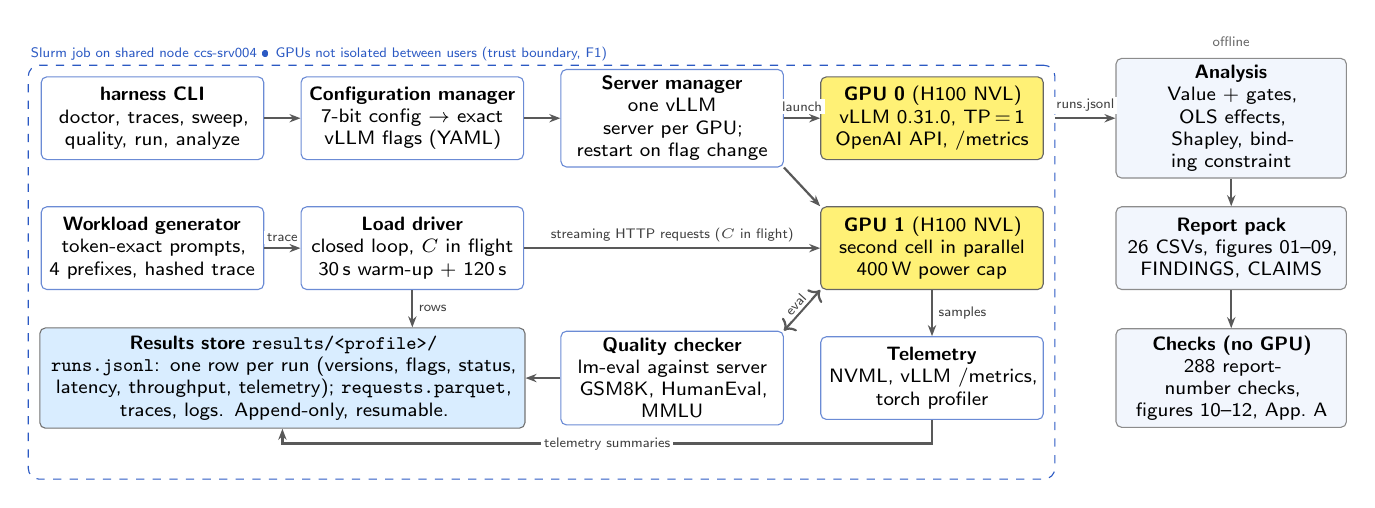
\begin{tikzpicture}[
  font=\sffamily\scriptsize,
  every node/.style={align=center},
  box/.style={draw=accent!70,fill=white,rounded corners=2pt,inner sep=2.5pt,text width=2.65cm,minimum height=1.05cm},
  gpu/.style={draw=black!60,fill=measbg,rounded corners=2pt,inner sep=2.5pt,text width=2.65cm,minimum height=1.05cm},
  store/.style={draw=black!55,fill=openbg!70,rounded corners=2pt,inner sep=3pt,minimum height=1.05cm},
  off/.style={draw=black!45,fill=rowgray,rounded corners=2pt,inner sep=2.5pt,text width=2.75cm,minimum height=1.05cm},
  arr/.style={-{Stealth[length=4pt]},draw=black!65,thick},
  lab/.style={font=\sffamily\tiny,text=black!75,fill=white,inner sep=1pt}
]
\def\cA{1.45}\def\cB{4.75}\def\cC{8.05}\def\cD{11.35}\def\cE{15.15}
\def\rA{0}\def\rB{-1.65}\def\rC{-3.3}
% node-internal components
\node[box] (cli) at (\cA,\rA) {\textbf{harness CLI}\\doctor, traces, sweep,\\quality, run, analyze};
\node[box] (cfg) at (\cB,\rA) {\textbf{Configuration manager}\\7-bit config $\to$ exact\\vLLM flags (YAML)};
\node[box] (srv) at (\cC,\rA) {\textbf{Server manager}\\one vLLM server per GPU;\\restart on flag change};
\node[gpu] (g0)  at (\cD,\rA) {\textbf{GPU 0} (H100 NVL)\\vLLM 0.31.0, TP\,=\,1\\OpenAI API, /metrics};
\node[box] (wl)  at (\cA,\rB) {\textbf{Workload generator}\\token-exact prompts,\\4 prefixes, hashed trace};
\node[box] (ld)  at (\cB,\rB) {\textbf{Load driver}\\closed loop, $C$ in flight\\30\,s warm-up + 120\,s};
\node[gpu] (g1)  at (\cD,\rB) {\textbf{GPU 1} (H100 NVL)\\second cell in parallel\\400\,W power cap};
\node[store,text width=5.95cm] (rs) at ($(\cA,\rC)!0.5!(\cB,\rC)$)
  {\textbf{Results store} \texttt{results/<profile>/}\\\texttt{runs.jsonl}: one row per run (versions, flags, status,
  latency, throughput, telemetry); \texttt{requests.parquet}, traces, logs. Append-only, resumable.};
\node[box] (q)   at (\cC,\rC) {\textbf{Quality checker}\\lm-eval against server\\GSM8K, HumanEval,\\MMLU};
\node[box] (tel) at (\cD,\rC) {\textbf{Telemetry}\\NVML, vLLM /metrics,\\torch profiler};
\coordinate (bot) at ($(rs.south)+(0,-0.5)$);
\begin{scope}[on background layer]
\node[draw=accent,dashed,rounded corners=4pt,fit=(cli)(g0)(rs)(tel)(bot),inner sep=4pt] (frame) {};
\node[anchor=south west,font=\sffamily\tiny,text=accent,inner sep=1pt] at (frame.north west)
  {Slurm job on shared node ccs-srv004 \textbullet\ GPUs not isolated between users (trust boundary, F1)};
\end{scope}
% offline column
\node[off] (an)  at (\cE,\rA) {\textbf{Analysis}\\Value + gates, OLS effects,\\Shapley, binding constraint};
\node[off] (rp)  at (\cE,\rB) {\textbf{Report pack}\\26 CSVs, figures 01--09,\\FINDINGS, CLAIMS};
\node[off] (ver) at (\cE,\rC) {\textbf{Checks (no GPU)}\\288 report-number checks,\\figures 10--12, App.\ A};
\node[font=\sffamily\tiny,text=black!60,anchor=south] at ($(an.north)+(0,0.02)$) {offline};
% arrows
\draw[arr] (cli) -- (cfg);
\draw[arr] (cfg) -- (srv);
\draw[arr] (srv) -- node[lab,above=1pt]{launch} (g0);
\draw[arr] (srv.south east) -- (g1.north west);
\draw[arr] (wl) -- node[lab,above=1pt]{trace} (ld);
\draw[arr] (ld) -- node[lab,above=1pt]{streaming HTTP requests ($C$ in flight)} (g1);
\draw[arr,<->] (q.north east) -- node[lab,sloped,above=0pt]{eval} (g1.south west);
\draw[arr] (g1) -- node[lab,right=1pt]{samples} (tel);
\draw[arr] (ld) -- node[lab,right=1pt]{rows} (ld |- rs.north);
\draw[arr] (q) -- (rs);
\draw[arr] (tel.south) -- ++(0,-0.3) -| node[lab,pos=0.25]{telemetry summaries} (rs.south);
\draw[arr] (an) -- (rp);
\draw[arr] (rp) -- (ver);
\draw[arr] (frame.east |- g0) -- node[lab,above=1pt]{runs.jsonl} (an.west);
\end{tikzpicture}
\caption{Components and data flow. Everything inside the dashed box runs in one Slurm job on the shared GPU node;
the grey column runs offline on the exported results. Model weights and the EAGLE-3 head are downloaded
from the public Hugging Face Hub (no token).}
\label{fig:arch}
\end{figure}

\begin{table}[H]
\small
{\rowcolors{2}{white}{rowgray}
\begin{tabularx}{\linewidth}{@{}P{3.1cm}LP{4.6cm}@{}}
\toprule
\rowcolor{tblhead}\hc{Component} & \hc{Responsibility} & \hc{Interface / data} \\
\midrule
CLI / orchestrator & Runs the study in order (doctor, traces, sweep, startup-check, quality, run, analyze;
\texttt{pipeline} runs them all); groups runs by engine flags to minimise restarts; failures become result rows
(ADR-011). & \fp{python -m harness <cmd> --profile <fast|investigate> --env h100}; \fp{harness/orchestrator.py} \\
Configuration manager & Validates YAML (pydantic, unknown keys rejected); maps a 7-bit configuration to exact
\texttt{vllm serve} flags in one file. & \fp{configs/experiment.yaml}, \fp{configs/env/h100.yaml},
\fp{harness/engine/vllm_flags.py} \\
Server manager & One \texttt{vllm serve} per GPU slot with its own port; classifies start-up failures (OOM,
unsupported, timeout, port in use); reads effective settings back; resets the prefix cache between reps. &
\fp{harness/engine/vllm_server.py}; \texttt{/metrics}, dev-mode \texttt{/server\_info} \\
Workload generator & Seeded random-word prompts sent as token IDs (exact lengths), 4 pooled prefixes; one saved,
hashed trace per point (ADR-005). & \fp{harness/workload.py}; seed 20261029 \\
Load driver & Async closed-loop client keeping $C$ requests in flight; client-side TTFT/TPOT; only requests that
start and finish in the window count. & \fp{harness/load_driver.py}; streaming \texttt{/v1/completions} \\
Telemetry & NVML (utilisation, clocks, power, memory, throttle reasons) and vLLM metrics through a fallback name
table; phase-2 time series and profiler parsing (ADR-010). & \fp{harness/telemetry.py},
\fp{harness/deep_telemetry.py} \\
Quality checker & lm-eval against the running server once per numeric setting; per-question answers for paired
tests (ADR-009, 018). & \fp{harness/quality.py} \\
Analysis & Value and gates, OLS effects and interactions, exact Shapley shares, binding label, investigation report.
& \fp{harness/analysis/} \\
Checks and figures & Re-derive every report number and figures 10--12 from the exported CSVs (ADR-020). &
\fp{evaluation/check_report_numbers.py}, \fp{evaluation/make_report_figures.py} \\
\bottomrule
\end{tabularx}}
\end{table}

\textbf{Data model.} One row per run in \fp{runs.jsonl}, keyed by \texttt{profile\_\_env\_\_point\_\_bits\_\_rep},
with versions, exact flags, engine-reported settings, trace hash, seed, status
(\texttt{ok}/\texttt{infeasible}/\texttt{failed}/\texttt{timeout}), throughput, latency percentiles and telemetry.
The latest row per key wins, so every command resumes where it stopped. The report pack exports these rows as CSVs
documented in \fp{DATA_DICTIONARY.md} (e.g.\ \fp{data/runs_combined_clean.csv}, 363 runs \x\ 107 columns).
\textbf{Security and trust boundaries.} (i) The GPU node is shared and does not isolate GPUs; another user's process
silently shared GPU\,0 during phase 1 (\S\ref{sec:contam}, ADR-015). (ii) HumanEval executes model-written code; the harness runs it
through lm-eval in the measurement job, without a sandbox (ADR-009), a risk listed in \S8.
(iii) \texttt{VLLM\_SERVER\_DEV\_MODE=1} exposes reset/info endpoints; servers use a per-job port range. No secrets or
personal data are used. \textbf{Decisions:} 21 records, ADR-000 (the 9 October methodology record) to ADR-020.

% =====================================================================
\section{Methodology \& experiment setup}
% =====================================================================
\textbf{Evaluation questions.} EQ1: how much does each optimization raise throughput in each regime? EQ2: do
optimizations add, multiply or cancel? EQ3: which configuration is best per workload under the gates, and what
binds it? EQ4: where and why does each optimization stop helping? EQ5: does any optimization degrade output quality?
EQ6: are the measurements trustworthy?

\begin{table}[H]
\small
{\rowcolors{2}{white}{rowgray}
\begin{tabularx}{\linewidth}{@{}>{\bfseries\raggedright\arraybackslash}p{3.2cm}L@{}}
\toprule
\rowcolor{tblhead}\hc{Item} & \hc{Setting} \\
\midrule
Hardware & 1 Slurm node, 2\,\x\,NVIDIA H100 NVL 94\,GB (compute capability 9.0, 400\,W power limit, PCIe), 16 CPU
cores per job; driver 590.48.01. It replaced the project's 4\,\x\,RTX 6000 Ada (48\,GB) node on 5 Nov (ADR-014) \\
Software & vLLM 0.31.0+cu129, PyTorch 2.13.0+cu129 (recorded in all 510 rows), FlashInfer 0.7.0.post1, lm-eval
0.4.13. On the cluster these pinned wheels ran in a conda environment (Python 3.10, cluster \texttt{nvcc} 13.1 for
FlashInfer's JIT kernels; \fp{cluster/}), not the \fp{scripts/setup_env.sh} venv (ADR-001, ADR-014) \\
Model \& engine args & \fp{unsloth/Llama-3.1-8B-Instruct}, \fp{--max-model-len 16384},
\fp{--gpu-memory-utilization 0.9}, \fp{--seed 20261029}, TP\,=\,1 \\
Optimizations & \opt{quant}: \fp{--quantization fp8} (W8A8, online dynamic); \opt{kvq}: \fp{--kv-cache-dtype fp8};
\opt{spec}: EAGLE-3, 3 draft tokens; \opt{prefix}: \fp{--enable-prefix-caching}; \opt{batch}:
\fp{--max-num-seqs} from a 16--256 sweep \\
Workload & Synthetic random-word prompts with exact token lengths; 4 shared prefixes = 75\% of a reusing prompt;
256-token outputs (\texttt{ignore\_eos}, greedy); closed loop with $C$ in flight. 7 points: centre (2048 tokens, 32
in flight, 50\% reuse) and one regime changed at a time. One hashed trace per point; 0 request errors in 510 runs
(\texttt{S4-trace}) \\
Phase 1 (factorial) & Full $2^5$ at the centre + even-parity $2^{5-1}$ half-fraction at 6 points = 128 cells \x\ 3
reps = 384 runs; 7 Nov 2026, 03:23--14:52 UTC, one cell per GPU, two at a time \\
Phase 2 (investigation) & 60 cells chosen from phase-1 anomalies, 2--5 reps, deep telemetry = 126 runs; 11 Nov,
19:08--23:31 UTC; 18 torch-profiler passes of 64 engine steps (ADR-016) \\
Measurement & 30\,s warm-up discarded, then a 120\,s window. Throughput = output tokens/s in the window; TTFT and
TPOT p50/p99 client-side. Cell value = geometric mean of reps \\
Accuracy & Phase 1: GSM8K 500, HumanEval 164, 4 MMLU subjects for the 8 numeric settings. Re-test: full GSM8K
(1,319), HumanEval (164), 8 MMLU subjects (1,687), paired with Default; McNemar test \cite{mcnemar}, paired 95\% CI \\
Analysis & OLS on log throughput, $\pm1$ coding, per point \cite{box}; interaction ratio
$I_{AB}=T_{AB}T_0/(T_AT_B)$; Shapley shares \cite{shapley} of the final configuration's log gain; binding constraint
from NVML, profiler and vLLM metrics \\
\bottomrule
\end{tabularx}}
\end{table}

\textbf{Run commands:}
\begin{codebox}
\footnotesize
\begin{verbatim}
scripts/setup_env.sh && scripts/slurm/prefetch.sh                # set-up
scripts/slurm/submit.sh 3        # phase 1: chained jobs, each running the line below
python -m harness pipeline --profile fast --env h100
python -m harness pipeline --profile investigate --env h100      # phase 2 (+ quality, analyze)
pytest tests/                                                    # no GPU: 69 unit tests
python -m harness pipeline --profile dry --env main --dry-run    # no GPU: simulated engine
python evaluation/check_report_numbers.py                        # no GPU: report numbers
python evaluation/make_report_figures.py                         # no GPU: figs 10-12, App. A
\end{verbatim}
\end{codebox}

% =====================================================================
\section{Results, observations \& analysis}
% =====================================================================
\subsection{Baseline versus submitted system}
\meas Default versus the best configuration that passes every gate under the original accuracy rule (\emph{policy
A}). No cell failed a latency gate; all 86 gate failures were accuracy failures (\texttt{S5.1-gates}).
\emph{Policy B} uses the paired re-test (\S\ref{sec:quality}) and is an upper bound, because its winners contain
FP8 weights + EAGLE-3, which was not paired-tested (ADR-018). Checks \texttt{S5.1-*}.

\begin{table}[H]
\small
\setlength{\tabcolsep}{4pt}
\begin{tabularx}{\linewidth}{@{}P{2.9cm}rrP{2.6cm}rr>{\bfseries}rL@{}}
\toprule
\rowcolor{tblhead}\hc{Workload} & \multicolumn{2}{c}{\hc{Default}} & \hc{Best (policy A)} & \multicolumn{2}{c}{\hc{Best}} & \hc{Speedup} & \hc{Policy B} \\

\cmidrule(lr){2-3}\cmidrule(lr){5-6}
\rowcolor{tblhead}\hc{(prompt $\cdot$ in flight $\cdot$ reuse)} & \hc{tok/s} & \hc{\makecell[r]{p99 TPOT /\\TTFT ms}} &   & \hc{tok/s} & \hc{\makecell[r]{p99 TPOT /\\TTFT ms}} &   & \hc{upper bound} \\
\midrule
Centre (2048 $\cdot$ 32 $\cdot$ 50\%) & 1,774 & 18.0 / 1,508 & spec+prefix & 3,231 & 16.6 / 326 & 1.82\x & 2.40\x \\
\rowcolor{rowgray} Short prompts (256) & 4,027 & 7.9 / 258 & spec+prefix & 7,777 & 8.6 / 67 & 1.93\x & 2.54\x \\
Long prompts (8192) & 495 & 59.2 / 1,038 & prefix+batch & 743 & 45.6 / 1,539 & 1.50\x & 1.82\x \\
\rowcolor{rowgray} Low concurrency (2) & 303 & 6.3 / 151 & spec+prefix & 753 & 4.2 / 122 & 2.48\x & 3.30\x \\
High concurrency (128) & 2,162 & 57.7 / 1,586 & spec+prefix & 3,602 & 60.4 / 891 & 1.67\x & 2.12\x \\
\rowcolor{rowgray} 0\% reuse & 1,776 & 17.8 / 1,500 & spec+prefix & 2,474 & 22.6 / 406 & 1.39\x & 1.39\x \\
90\% reuse & 1,775 & 17.7 / 1,785 & spec+prefix+batch & 4,657 & 12.1 / 199 & 2.62\x & 3.30\x \\
\bottomrule
\end{tabularx}
\caption{Baseline versus submitted system (\fp{data/cells_combined_clean.csv}, \fp{data/final_configs_by_policy.csv}).
Repetition CV $\le$ 1.53\% for every Default and best cell (2--3 reps).}
\end{table}

\begin{figure}[H]
\centering
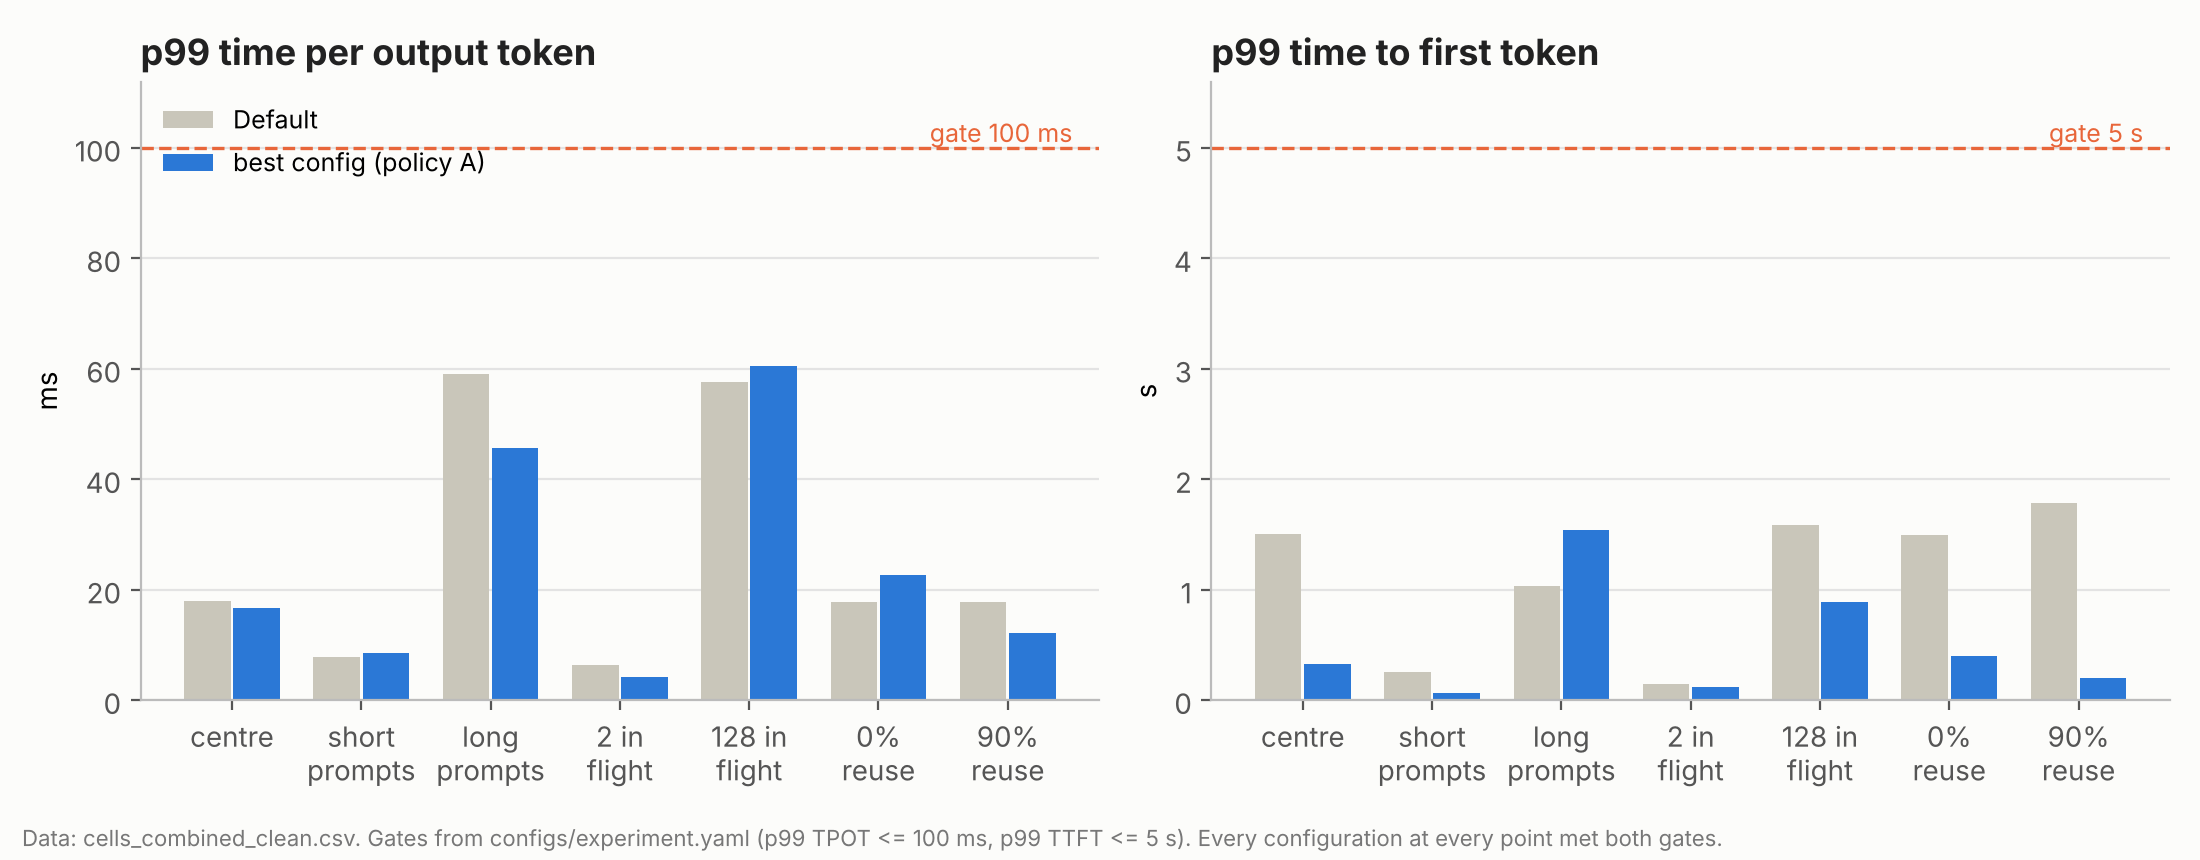
\includegraphics[width=0.88\linewidth]{figures/12_latency_vs_gates.png}
\caption{p99 latency of Default and of the policy-A winner at each workload, against the two latency gates.}
\end{figure}

spec + prefix (with or without tuned batching, which has no effect) wins at 6 of 7 workloads [C3]; at long prompts
prefix + batch wins because EAGLE-3 gives nothing there (\S\ref{sec:eagle}). Speculation shortens p99 TTFT sharply
but can lengthen p99 TPOT slightly (0\% reuse: 17.8 $\to$ 22.6\,ms), well inside the gate. Ignoring accuracy
(policy C) would add FP8 KV at the centre (2.48\x) and at long prompts (2.05\x).

\subsection{Critical failure found and fixed: hidden GPU interference (F1)}\label{sec:contam}
\begin{figure}[H]
\centering
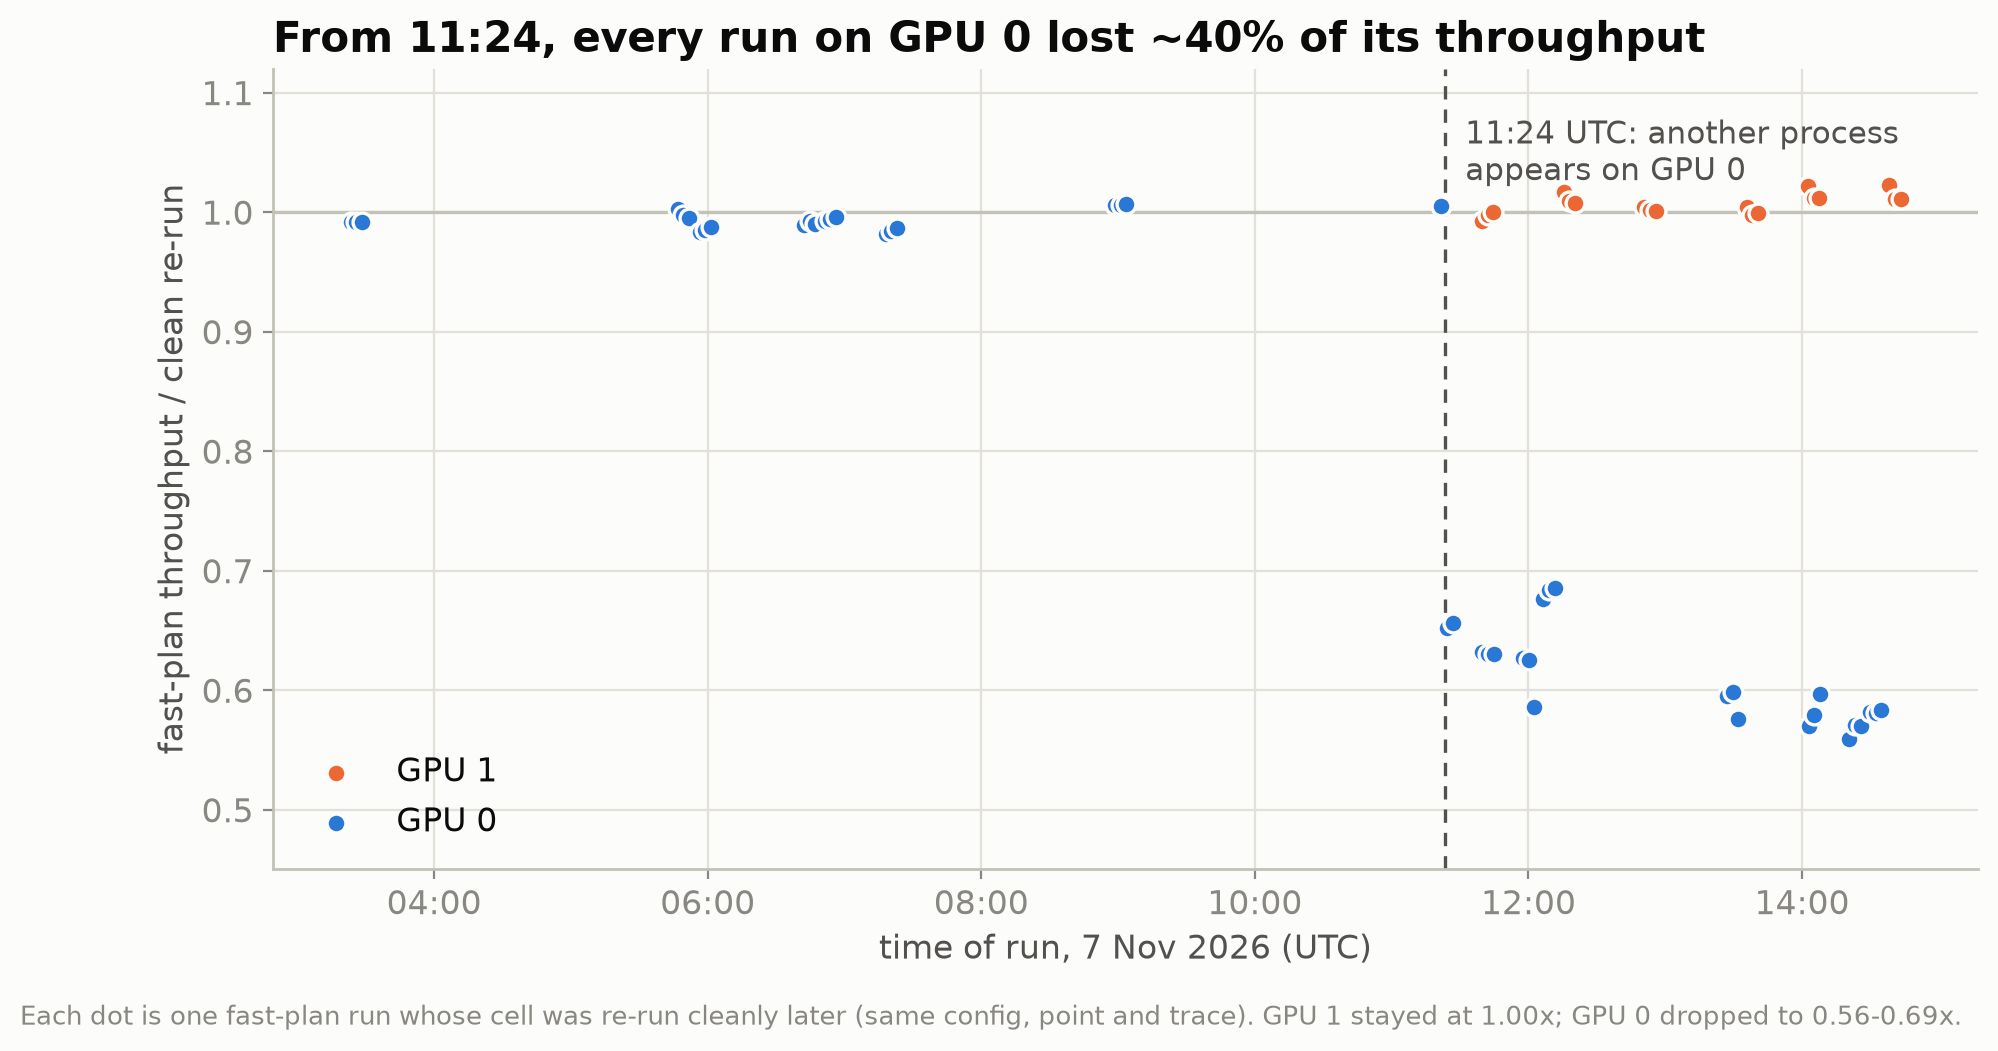
\includegraphics[width=0.49\linewidth]{figures/01_contamination_timeline.png}\hfill
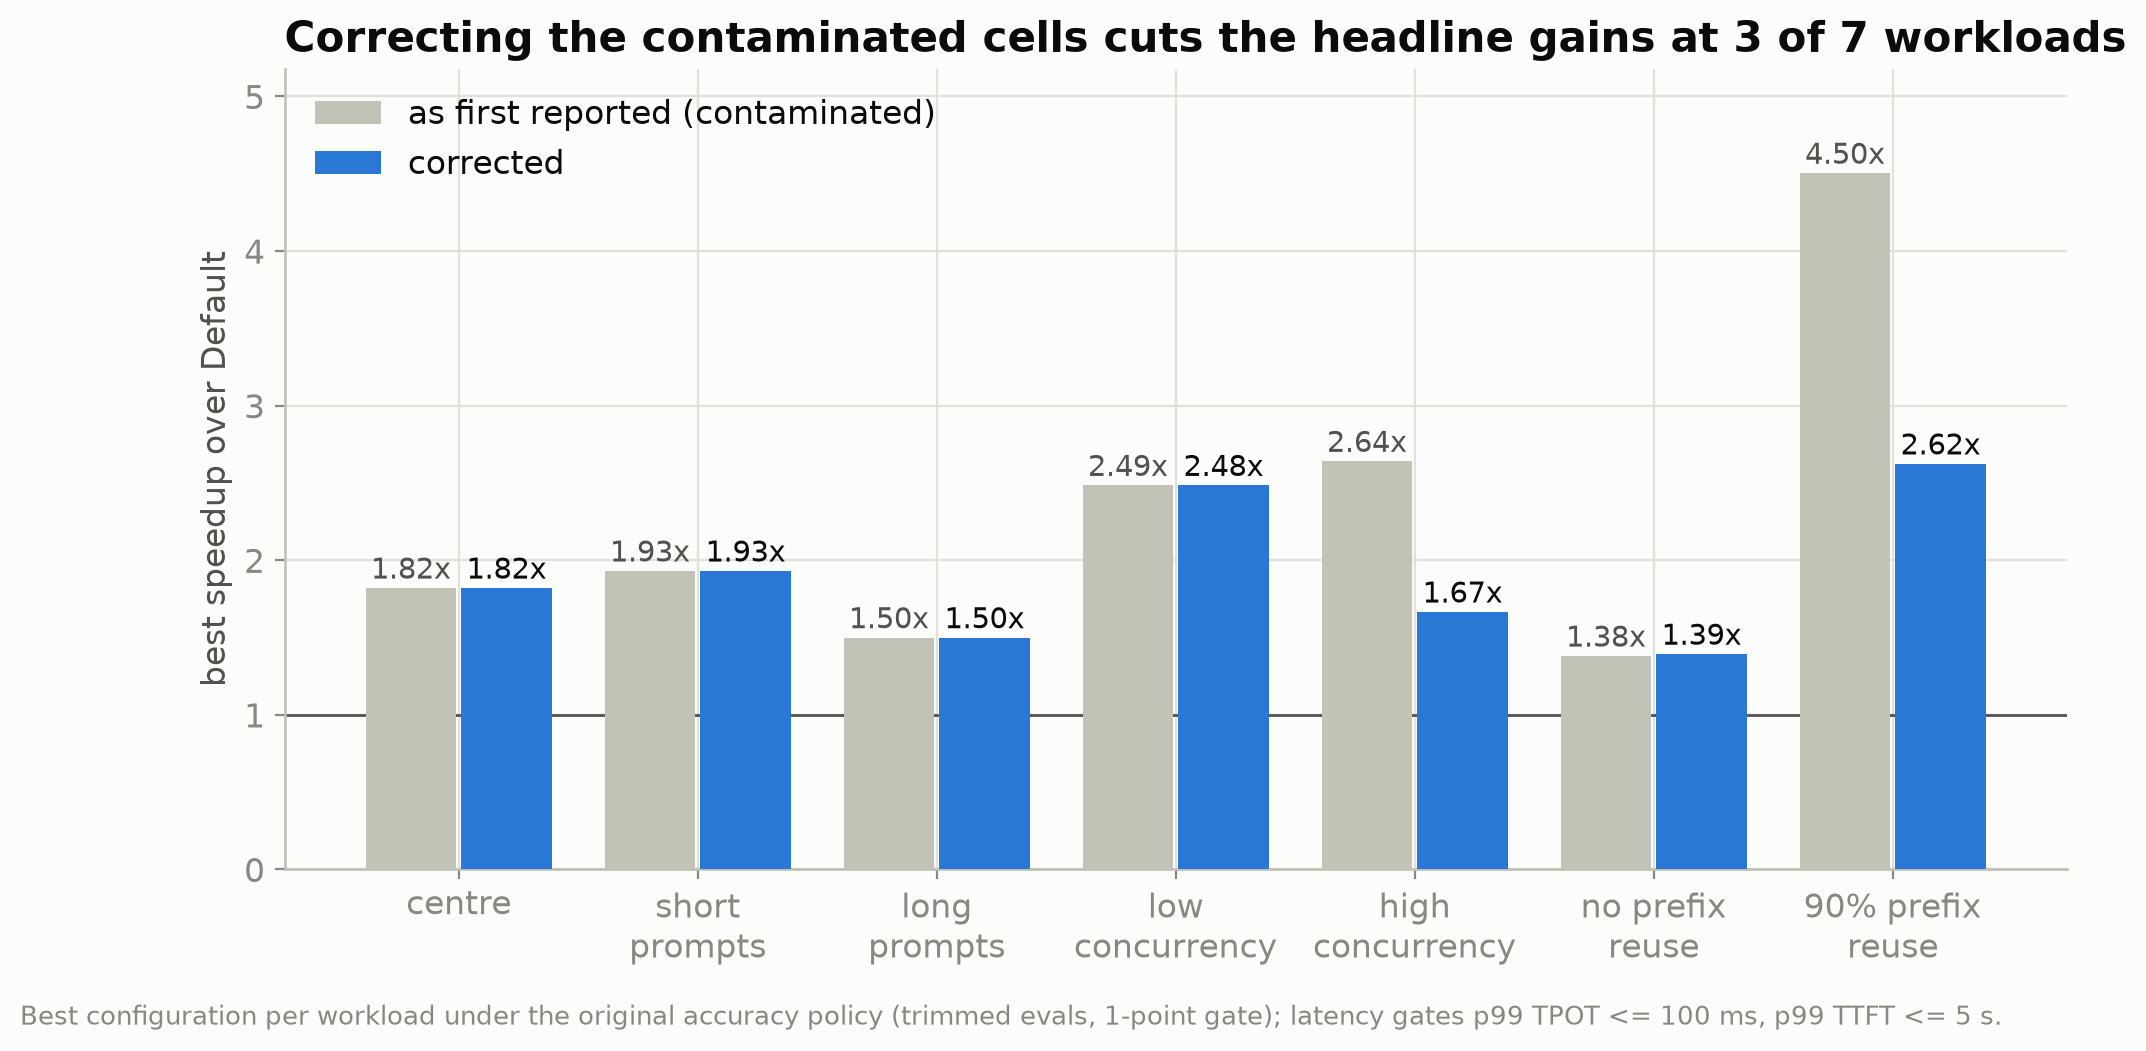
\includegraphics[width=0.49\linewidth]{figures/02_best_speedup_corrected.png}
\caption{Left: phase-1 throughput relative to a clean phase-2 re-run of the same cell, by time and GPU [C1]. Right:
best speedup per workload as first reported versus after removing the contaminated runs [C4].}
\end{figure}

\meas Comparing phase-2 re-runs with phase 1 showed that from 11:24 UTC on 7 Nov every run on GPU\,0 ran at
0.56--0.69\x\ its true throughput, while GPU\,1 stayed at 1.006\x. NVML recorded +4.3\,GB of device memory, a higher
SM clock and lower power on GPU\,0, the signature of another user's process sharing the GPU. 71 of 384 runs (18\%) in
24 cells were affected. Within a cell the slowdown was easy to miss: the 23 fully contaminated cells had a repetition
CV of 0.2--3.8\% (median 2.1\%), small next to a 40\% slowdown but ten times the 0.2\% median of the cleaned cells, a
signal a per-cell CV alarm could have caught; the pack's claim C2 (``$<$1\%'') is corrected here. \textbf{Correction} (ADR-017):
8 cells replaced by clean re-runs, 16 excluded (\fp{data/cells_missing_after_cleaning.csv}), 16 phase-2-only cells
added. The 40 uncontaminated phase-1 runs that were re-run match within 2.2\%. Best speedups fell from 4.50\x\ to
2.62\x\ (90\% reuse) and from 2.64\x\ to 1.67\x\ (high concurrency). Checks \texttt{S5.2}.

\begin{table}[H]
\small
{\rowcolors{2}{white}{rowgray}
\begin{tabularx}{\linewidth}{@{}Lrrrrr@{}}
\toprule
\rowcolor{tblhead}\hc{Phase} & \hc{Runs} & \hc{Median tok/s vs.\ clean re-run} & \hc{Device memory (MB)} & \hc{SM clock (MHz)} & \hc{Power (W)} \\
\midrule
GPU\,0 before 11:24 UTC & 124 & 0.992 & 87,498 & 1,172 & 396 \\
GPU\,0 from 11:24 UTC & 71 & \textbf{0.596} & 91,917 & 1,476 & 387 \\
GPU\,1 & 189 & 1.006 & 87,985 & 1,171 & 395 \\
\bottomrule
\end{tabularx}}
\end{table}

\subsection{Which optimization matters where (F8)}
\begin{figure}[H]
\centering
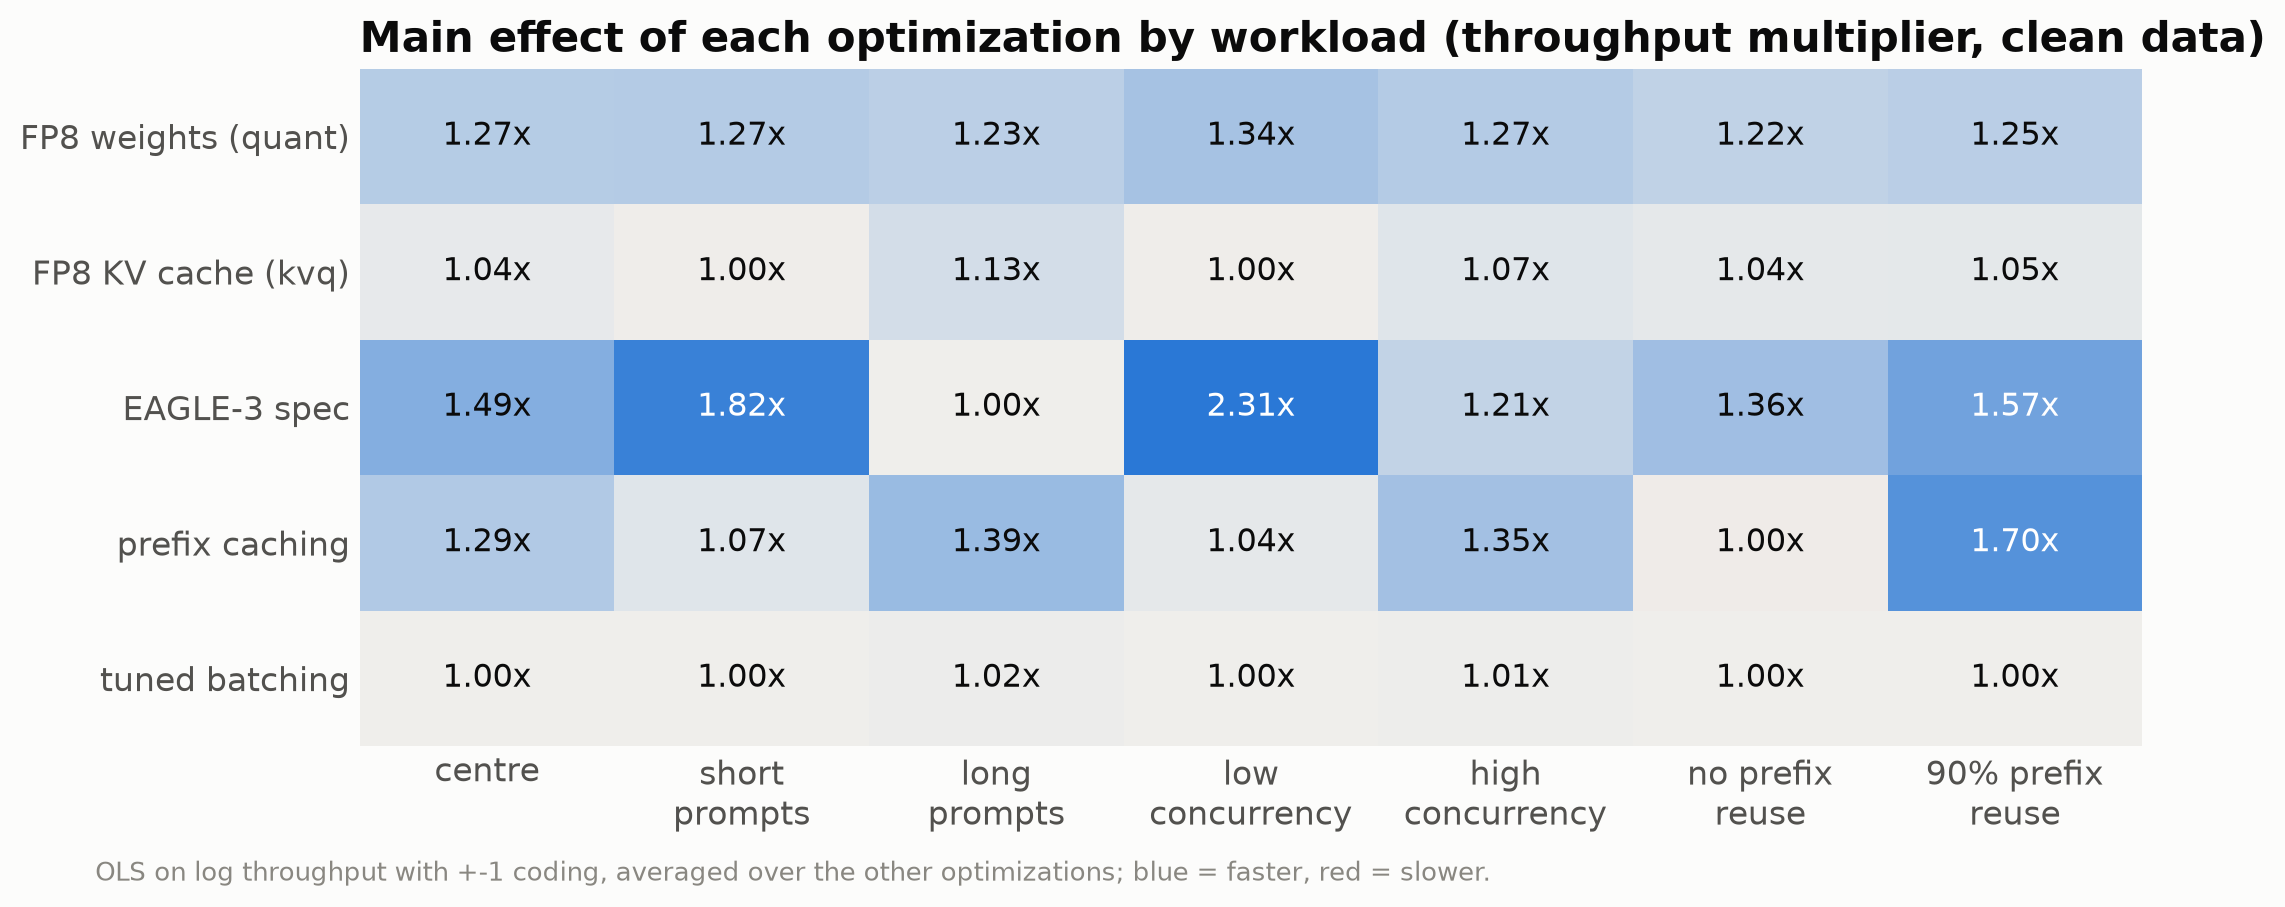
\includegraphics[width=0.92\linewidth]{figures/06_main_effects_heatmap.png}
\caption{Throughput multiplier of each optimization averaged over the others (OLS, $R^2 \ge 0.9976$ at every point;
\fp{data/clean_main_effects.csv}, checks \texttt{S5.3-*}).}
\end{figure}

\meas FP8 weights are the most consistent single lever (1.22--1.34\x\ everywhere). EAGLE-3 is the largest lever when
the GPU is under-used (2.31\x\ at 2 in flight) and useless on 8k-token prompts (1.00\x). Prefix caching tracks
reuse (1.00\x\ at 0\%, 1.70\x\ at 90\%). \textbf{No-benefit cases, with cause} (\fp{data/clean_no_benefit.csv}, 11
cases): \opt{batch} never helps (1.00--1.02\x) because the engine default of 256 sequences exceeds every in-flight
count [C14]; \opt{kvq} gives nothing where the KV cache is small ($\le$\,3\% used at short prompts and low
concurrency) and 1.13\x\ at long prompts where it is large; \opt{prefix} gives 1.00\x\ at 0\% reuse, with no
measurable tracking overhead.

\begin{figure}[H]
\centering
\begin{minipage}[c]{0.44\linewidth}
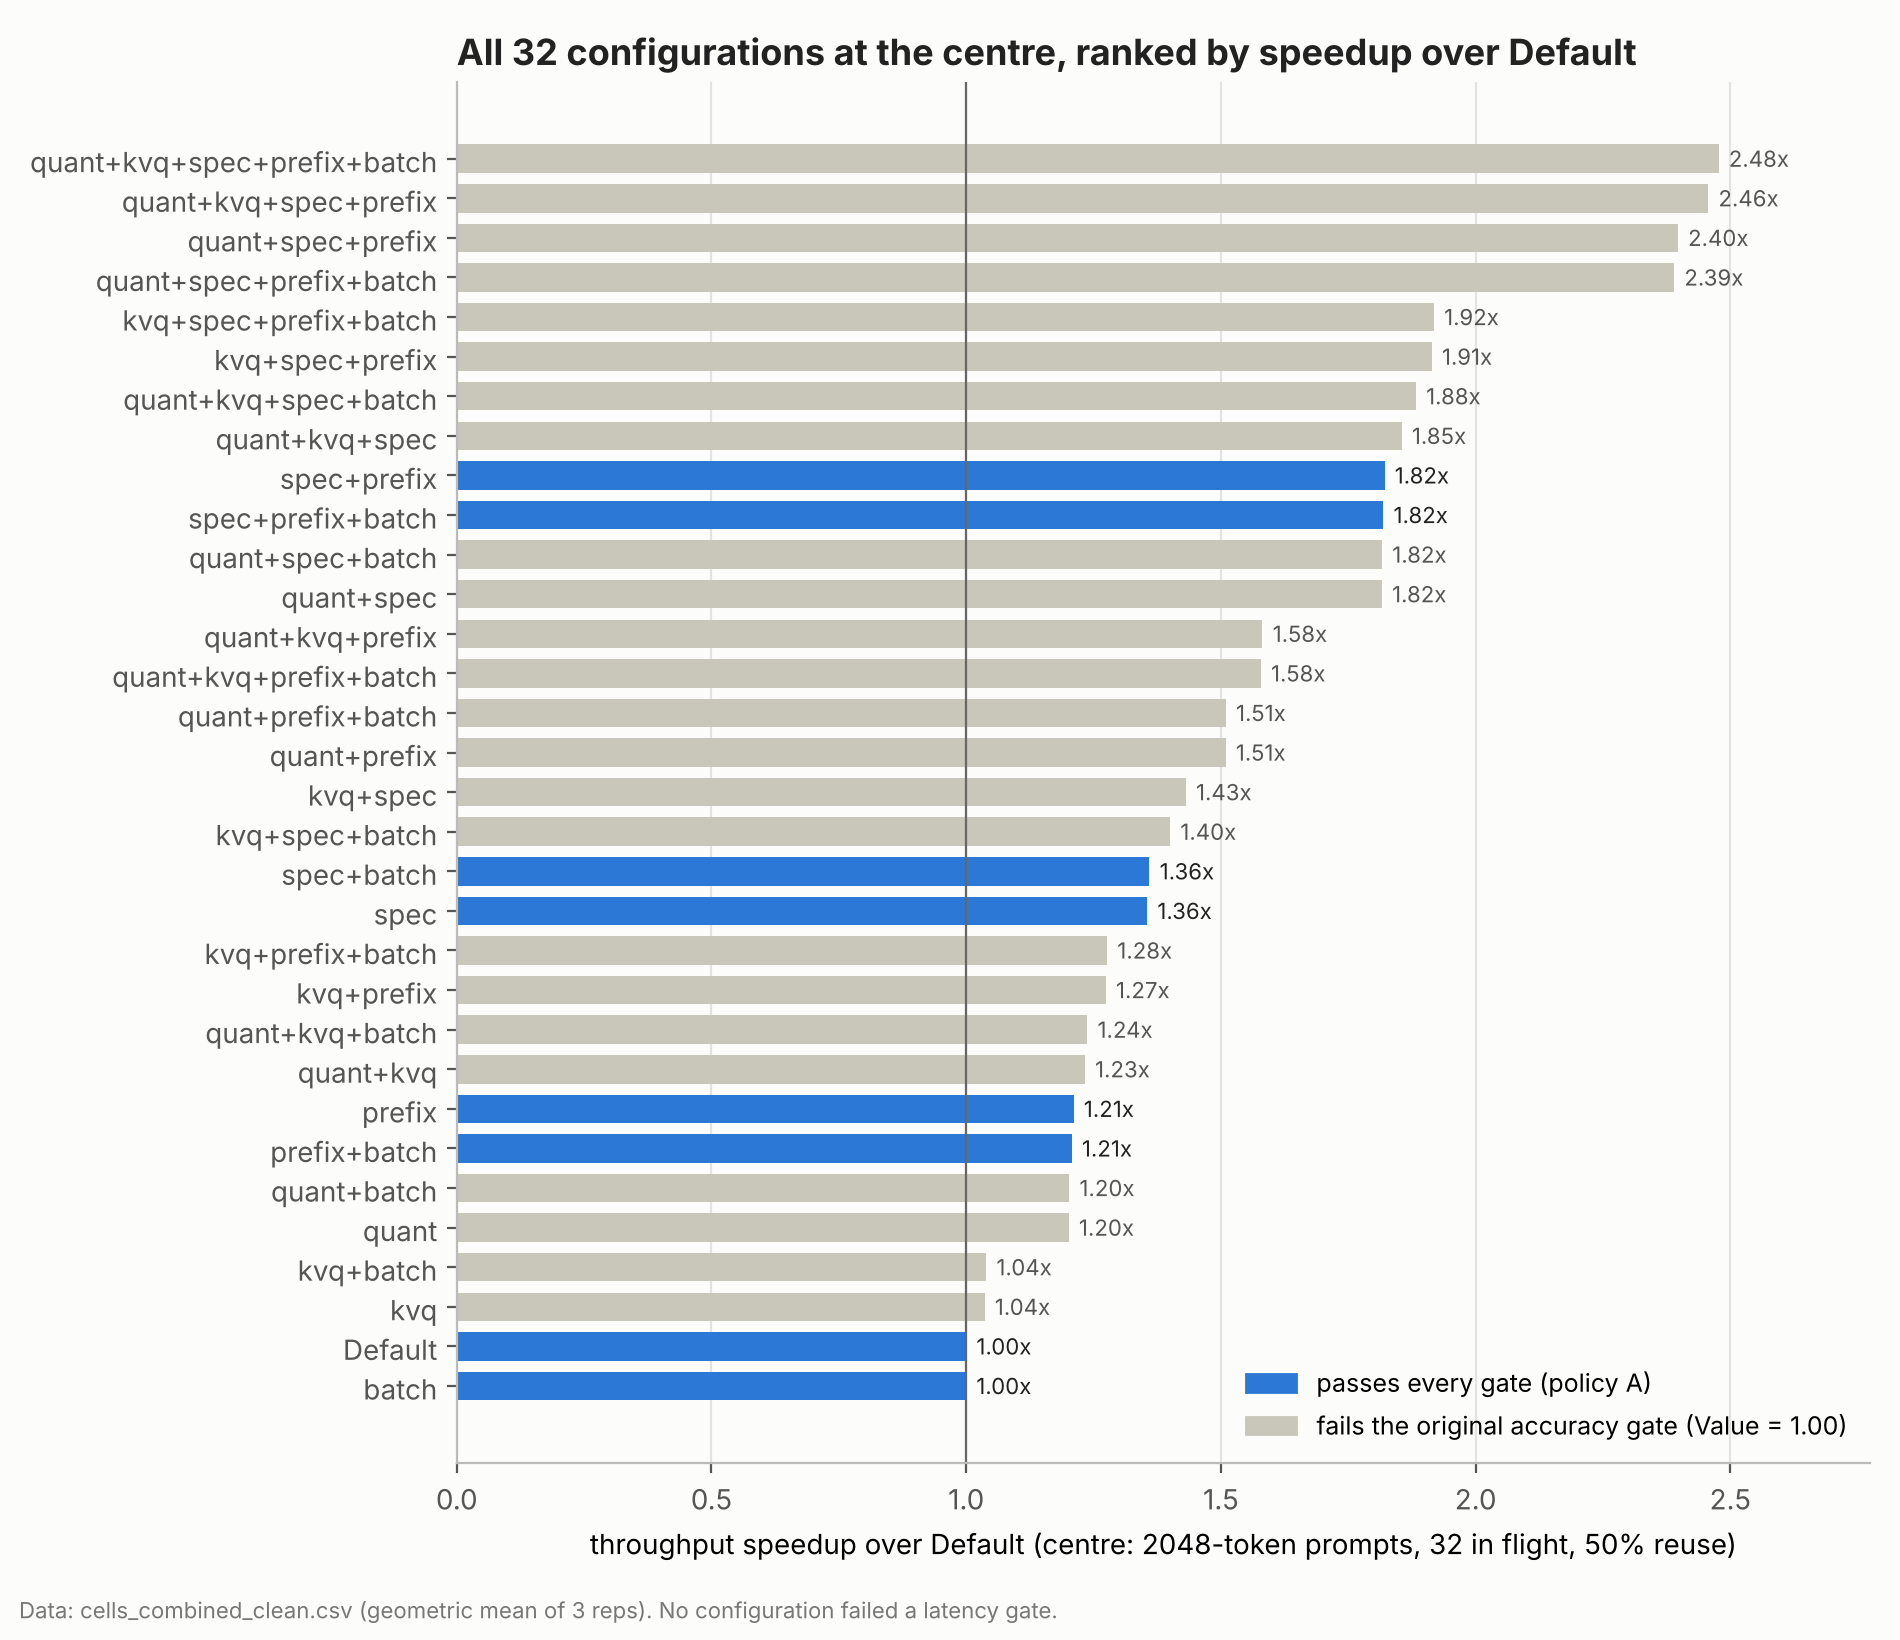
\includegraphics[width=\linewidth]{figures/10_centre_all_configs.png}
\end{minipage}\hfill
\begin{minipage}[c]{0.54\linewidth}
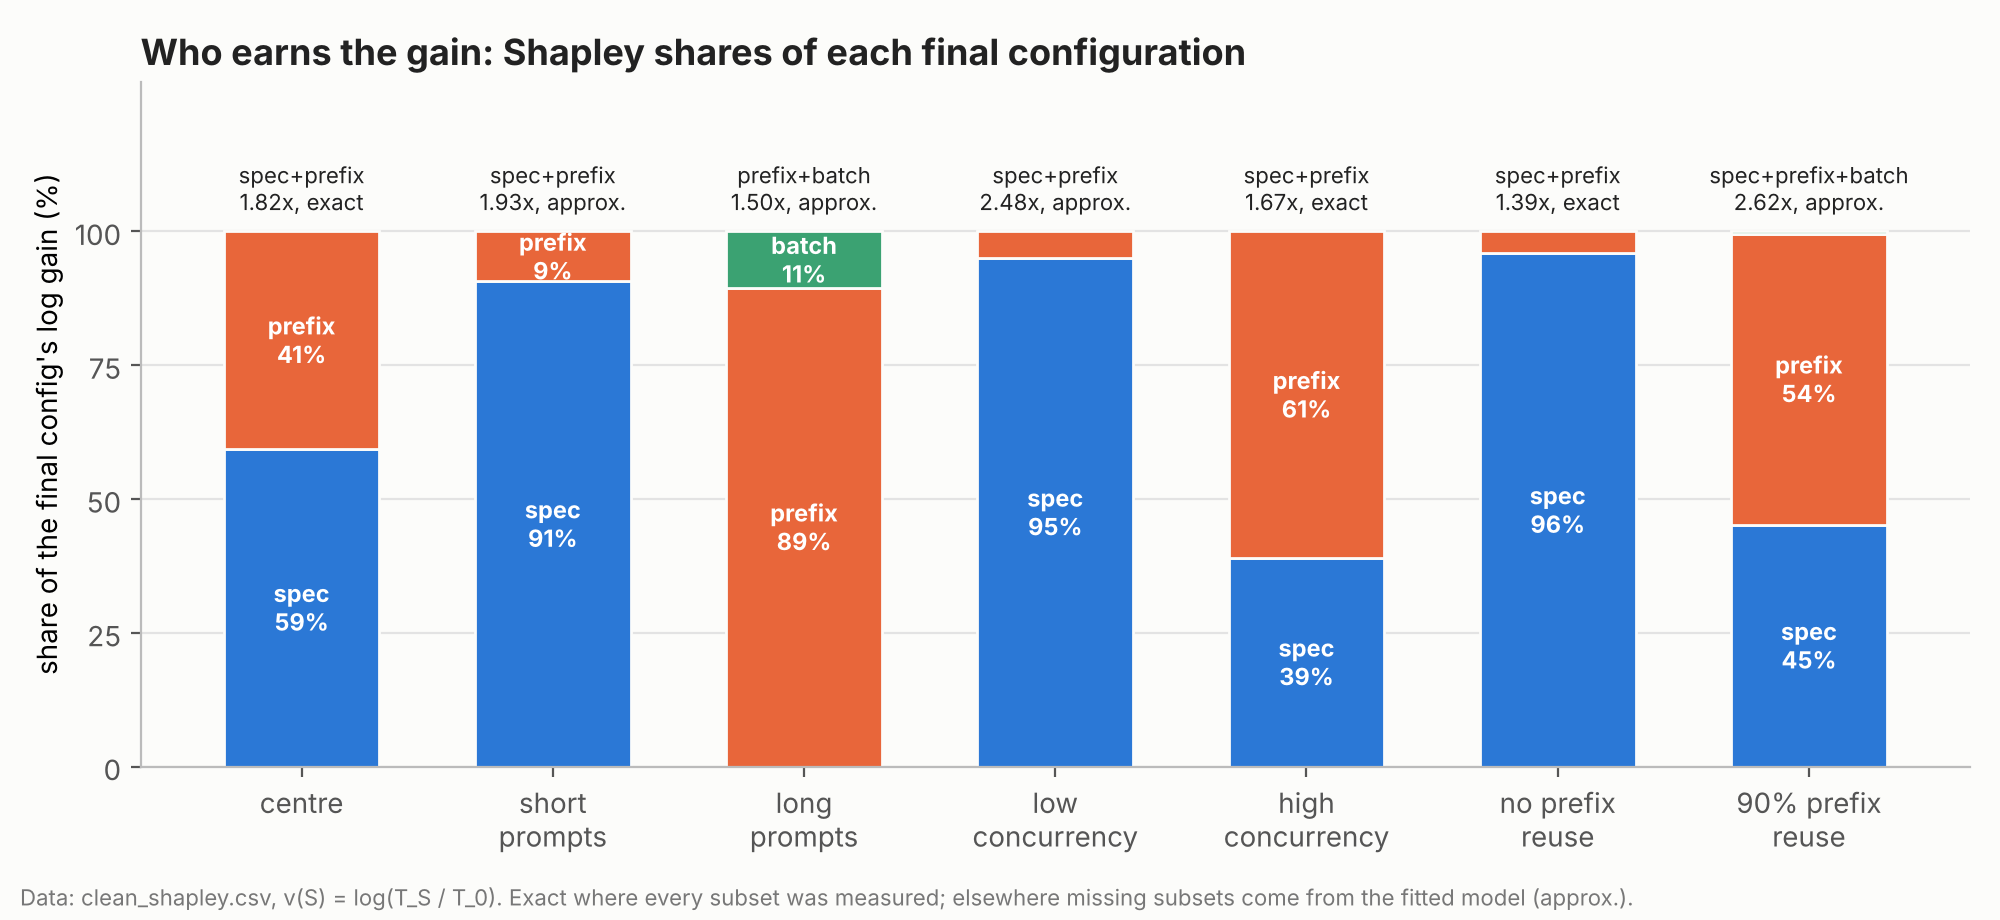
\includegraphics[width=\linewidth]{figures/11_shapley_shares.png}
\end{minipage}
\caption{Left: all 32 configurations at the centre; grey bars failed the original accuracy gate. Right: Shapley
shares of each final configuration's log gain (\fp{data/clean_shapley.csv}; exact at 3 points).}
\label{fig:centre}
\end{figure}

\meas At the centre the four fastest configurations all combine FP8 weights with spec and prefix (2.39--2.48\x), but
each contains an FP8 change that failed the phase-1 accuracy gate, so the policy-A winner is spec + prefix at 1.82\x\
(Figure~\ref{fig:centre}). Attribution of that winner: \opt{spec} 59\%, \opt{prefix} 41\% (exact). Where reuse is low
or the GPU is idle, \opt{spec} earns almost all of the gain (96\% at 0\% reuse, 95\% at 2 in flight); where many
requests share a prefix or the batch is large, \opt{prefix} dominates (61\% at 128 in flight, 89\% at long prompts).

\subsection{Combinations multiply, and with speculative decoding they compound (F3--F5)}
\begin{figure}[H]
\centering
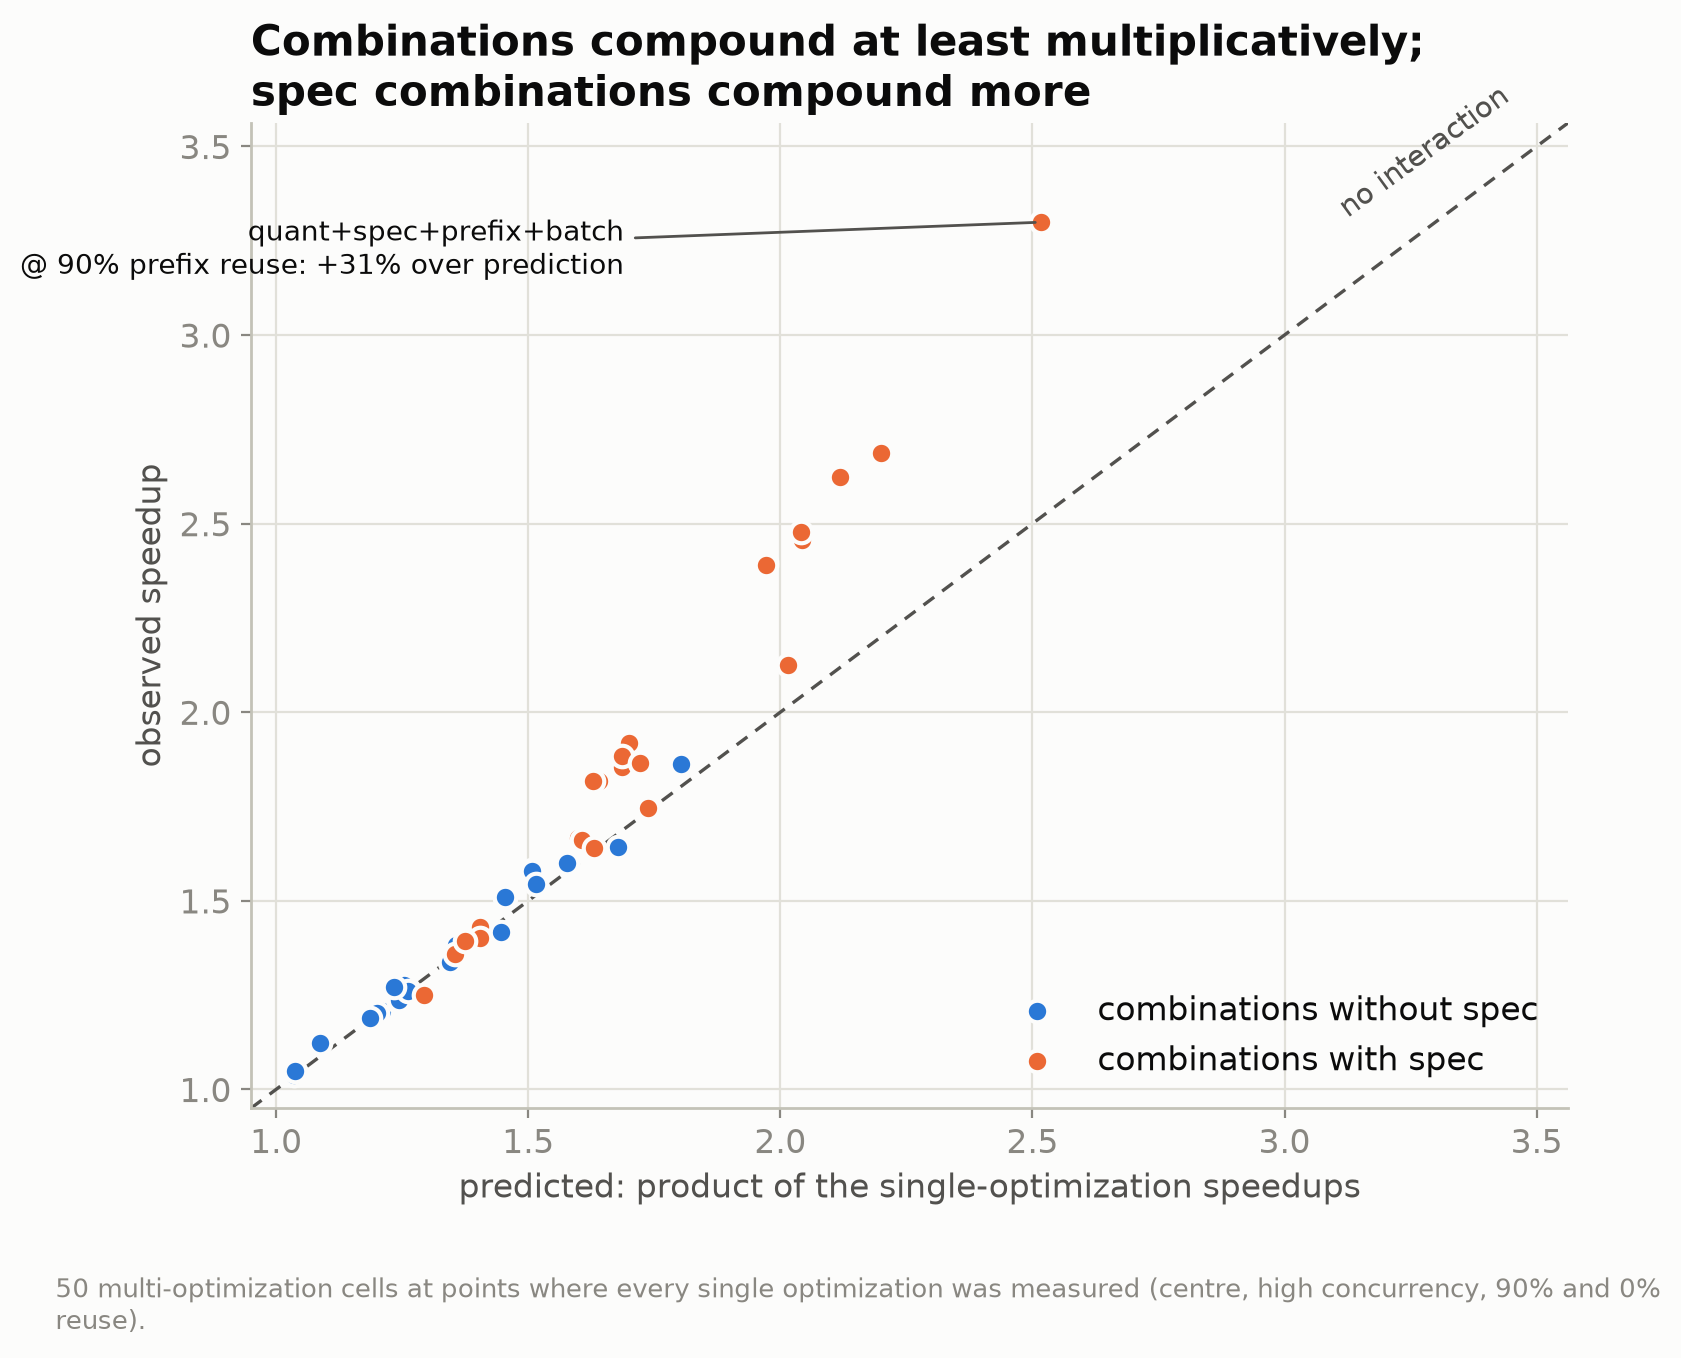
\includegraphics[width=0.42\linewidth]{figures/05_composition_observed_vs_predicted.png}\hfill
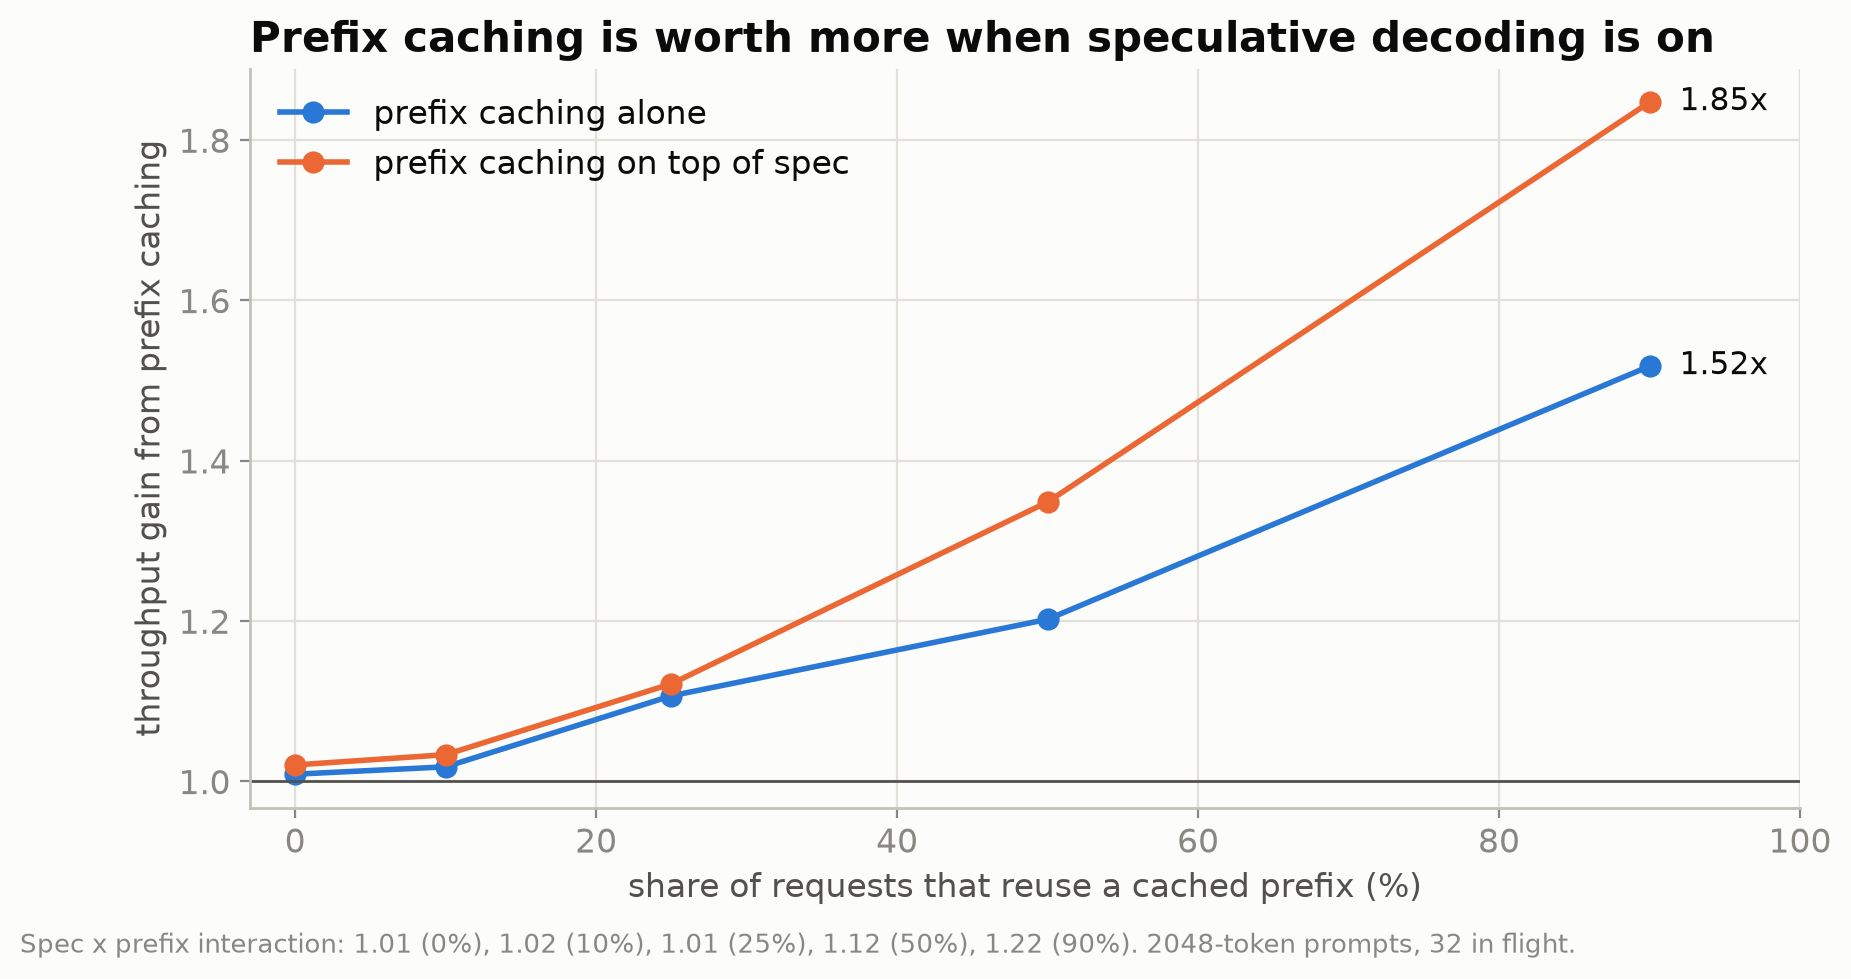
\includegraphics[width=0.54\linewidth]{figures/04_prefix_gain_vs_reuse.png}
\caption{Left: observed speedup versus the product of single-optimization speedups (50 combinations) [C5]. Right:
prefix-caching gain versus reuse, with and without EAGLE-3 [C7].}
\end{figure}

\meas For the 50 combinations whose single speedups were all measured, none fell more than 5\% below the product of
its parts; 32 matched it and 18 exceeded it by more than 5\%, all 18 containing \opt{spec}, up to +31\%
(quant+spec+prefix+batch at 90\% reuse). Mean observed/predicted: 1.111 with \opt{spec}, 1.013 without. At the centre
a multiplicative prediction has median error 4.8\% (max 21.6\%), an additive one 9.1\% (max 37.4\%):
\textbf{speedups multiply; they do not add} [C5, C6]. Checks \texttt{S5.4}.

\meas FP8 weights give 1.20\x\ alone but 1.34\x\ on top of EAGLE-3 at the centre (interaction 1.115); with \opt{spec}
each engine step processes 928 instead of 284 tokens [C9]. \interp verifying 3 draft tokens makes each step a larger
matrix multiply, where FP8 tensor-core math helps most [C10].

\meas The \opt{spec} \x\ \opt{prefix} interaction is 1.01 at 0--25\% reuse, 1.12 at 50\% and 1.22 at 90\%. At 90\%
reuse prefix caching shortens each request's decode phase by 27\% without \opt{spec} and by 45\% with it.
\interp (Amdahl's law \cite{amdahl}): vLLM mixes prompt processing and decoding in the same engine steps; \opt{spec}
shrinks the decode share, so the prompt share that prefix caching removes becomes larger [C8]. \open the threshold
between 25\% and 50\% reuse is not located.

\subsection{Where optimizations stop working: EAGLE-3 on long prompts (F6)}\label{sec:eagle}
\begin{figure}[H]
\centering
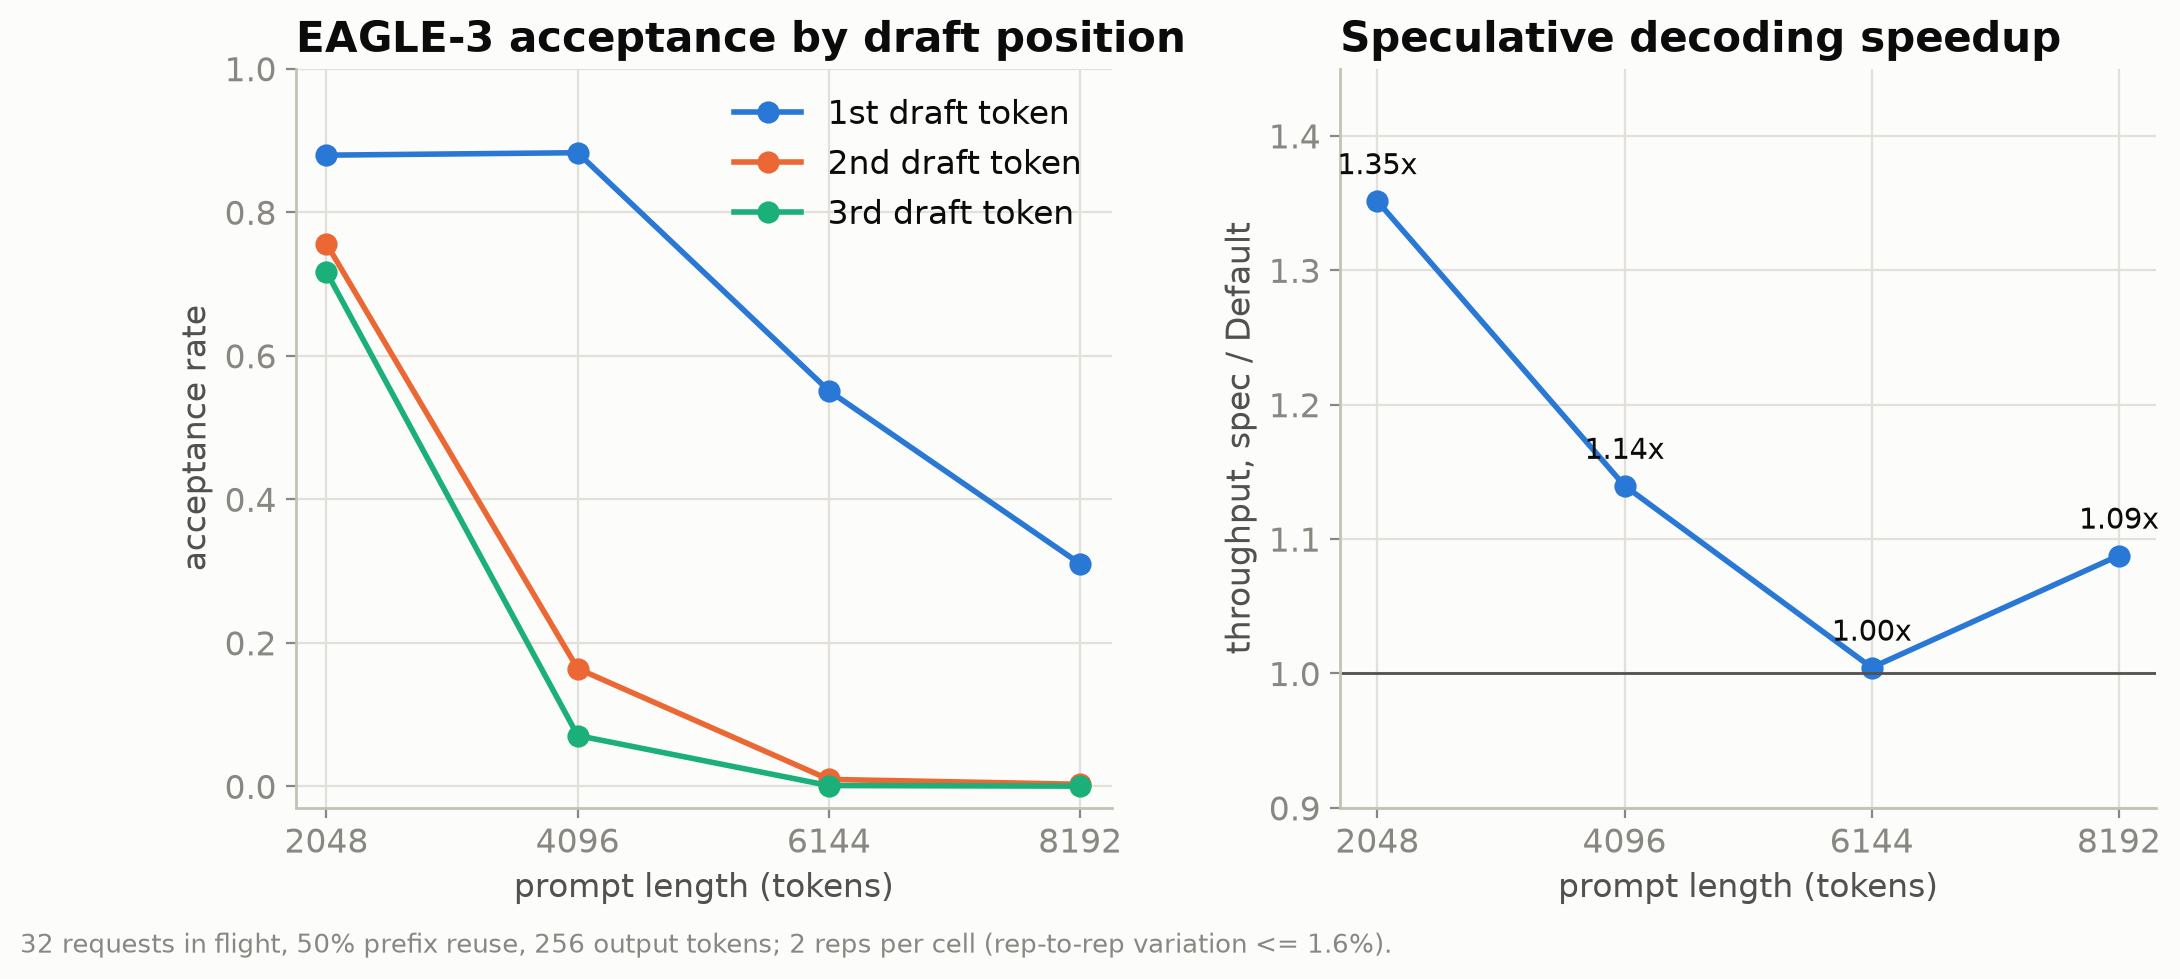
\includegraphics[width=0.80\linewidth]{figures/03_eagle3_long_context.png}
\caption{EAGLE-3 acceptance by draft position (left) and speedup versus prompt length (right) [C11].}
\end{figure}
\meas EAGLE-3's speedup falls from 1.35\x\ at 2,048-token prompts to 1.14\x\ at 4,096 and 1.00\x\ at 6,144;
acceptance of the 2nd draft token collapses from 0.76 to 0.16 between 2k and 4k (tokens per step 3.35 $\to$ 2.12
$\to$ 1.56). Checks \texttt{S5.5-*}. \interp (low confidence) the draft head was probably trained on shorter
contexts, so the positions that build on its own guesses fail first [C12]; its training length was not checked.
\textbf{Practical rule:} gate speculative decoding on prompt length (off beyond $\sim$4k tokens) or use a
long-context draft head. \open \opt{spec} also cuts median TTFT at the centre (1,046 $\to$ 183\,ms), which
speculation does not obviously explain.

\subsection{Output quality: an interaction between the two FP8 changes (F7)}\label{sec:quality}
\begin{figure}[H]
\centering
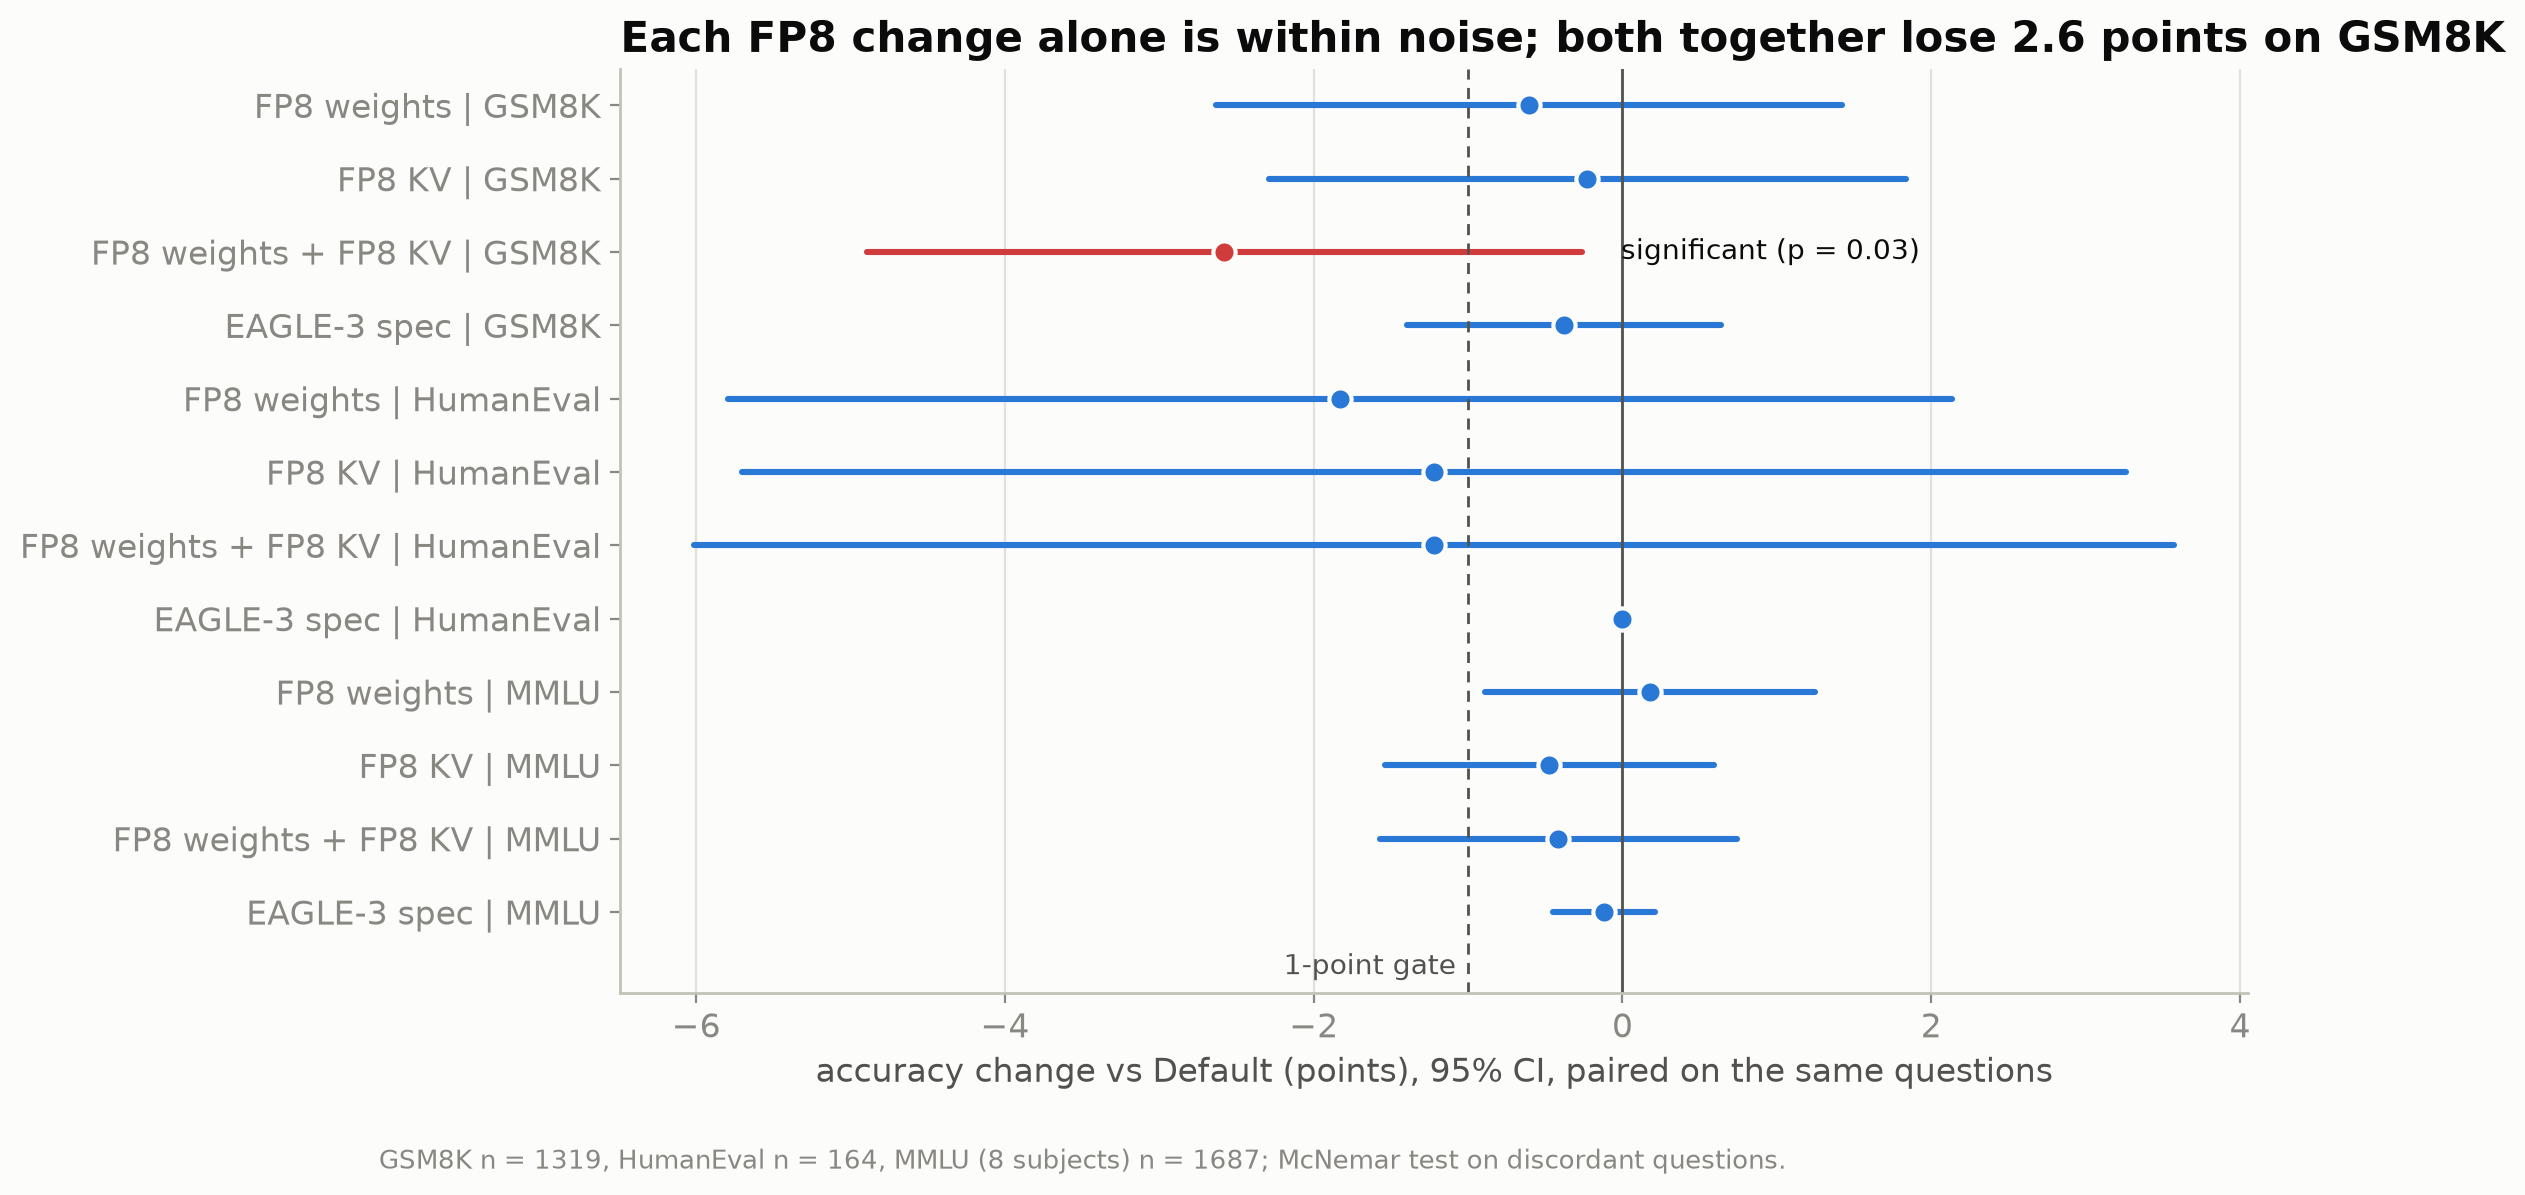
\includegraphics[width=0.74\linewidth]{figures/07_accuracy_paired.png}
\caption{Paired accuracy change versus Default with 95\% CI, on identical questions [C13].}
\end{figure}

\meas FP8 weights alone and FP8 KV alone are not distinguishable from BF16 on 1,319 GSM8K questions; together they
lose 2.58 points (95\% CI $-4.9$ to $-0.3$, $p = 0.03$), the only significant drop [C13]. EAGLE-3 changed the outcome
of 47 of 1,319 GSM8K questions (n.s.) and no HumanEval result. The trimmed phase-1 evaluation had excluded each FP8
change on its own (e.g.\ $-3.0$ points for FP8 weights on 164 HumanEval problems); the paired test can neither
confirm nor exclude a 1-point drop for either change alone (CIs too wide), so those exclusions are not supported by
the data, while the combination shows the only significant drop (ADR-018). \interp each FP8 change adds a small rounding error that
compounds over multi-step arithmetic. Caveat: one greedy run per setting; quant+spec, kvq+spec and all three were not
paired-tested.

\begin{table}[H]
\small
\setlength{\tabcolsep}{4pt}
{\rowcolors{2}{white}{rowgray}
\begin{tabularx}{\linewidth}{@{}llrrrcrL@{}}
\toprule
\rowcolor{tblhead}\hc{Setting} & \hc{Task ($n$)} & \hc{Default\,\%} & \hc{Setting\,\%} & \hc{$\Delta$ pts} & \hc{95\% CI} & \hc{McNemar $p$} & \hc{Verdict} \\
\midrule
quant & GSM8K (1,319) & 69.6 & 69.0 & $-0.61$ & [$-2.6$, $+1.4$] & 0.61 & n.s.; CI too wide \\
kvq & GSM8K (1,319) & 69.6 & 69.4 & $-0.23$ & [$-2.3$, $+1.8$] & 0.89 & n.s.; CI too wide \\
\rowcolor{fillbg!60} quant+kvq & GSM8K (1,319) & 69.6 & 67.0 & $\mathbf{-2.58}$ & [$-4.9$, $-0.3$] & 0.03 & \textbf{significant drop} \\
spec & GSM8K (1,319) & 69.6 & 69.2 & $-0.38$ & [$-1.4$, $+0.6$] & 0.56 & n.s.; CI too wide \\
quant & HumanEval (164) & 63.4 & 61.6 & $-1.83$ & [$-5.8$, $+2.1$] & 0.55 & n.s.; CI too wide \\
kvq & HumanEval (164) & 63.4 & 62.2 & $-1.22$ & [$-5.7$, $+3.3$] & 0.79 & n.s.; CI too wide \\
quant+kvq & HumanEval (164) & 63.4 & 62.2 & $-1.22$ & [$-6.0$, $+3.6$] & 0.80 & n.s.; CI too wide \\
spec & HumanEval (164) & 63.4 & 63.4 & $+0.00$ & [$+0.0$, $+0.0$] & 1.00 & within gate \\
quant & MMLU-8 (1,687) & 65.7 & 65.9 & $+0.18$ & [$-0.9$, $+1.2$] & 0.83 & within gate \\
kvq & MMLU-8 (1,687) & 65.7 & 65.3 & $-0.47$ & [$-1.5$, $+0.6$] & 0.45 & n.s.; CI too wide \\
quant+kvq & MMLU-8 (1,687) & 65.7 & 65.3 & $-0.41$ & [$-1.6$, $+0.7$] & 0.55 & n.s.; CI too wide \\
spec & MMLU-8 (1,687) & 65.7 & 65.6 & $-0.12$ & [$-0.4$, $+0.2$] & 0.73 & within gate \\
\bottomrule
\end{tabularx}}
\caption{Paired accuracy versus Default (\fp{data/quality_paired_vs_default.csv}; checks \texttt{S5.6-*}).}
\end{table}

\subsection{Binding constraint (F9) and measurement validity (F10)}
\begin{figure}[H]
\centering
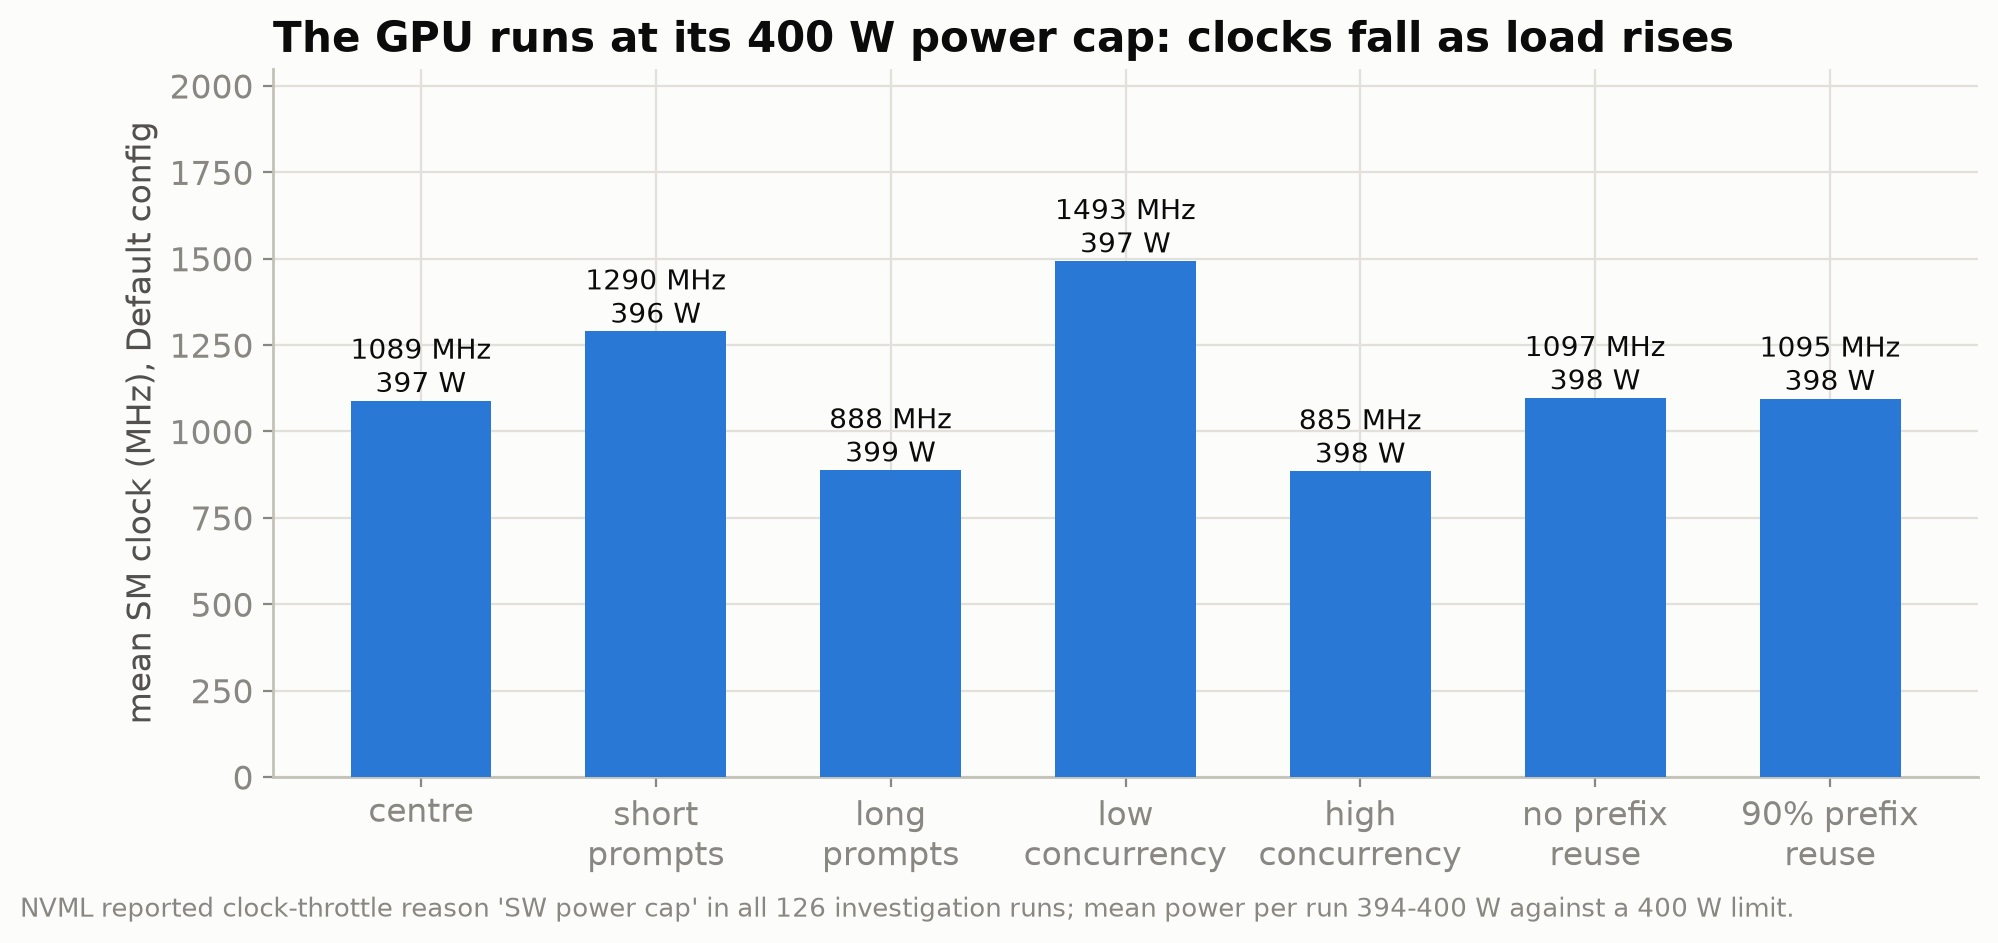
\includegraphics[width=0.49\linewidth]{figures/08_power_cap_clocks.png}\hfill
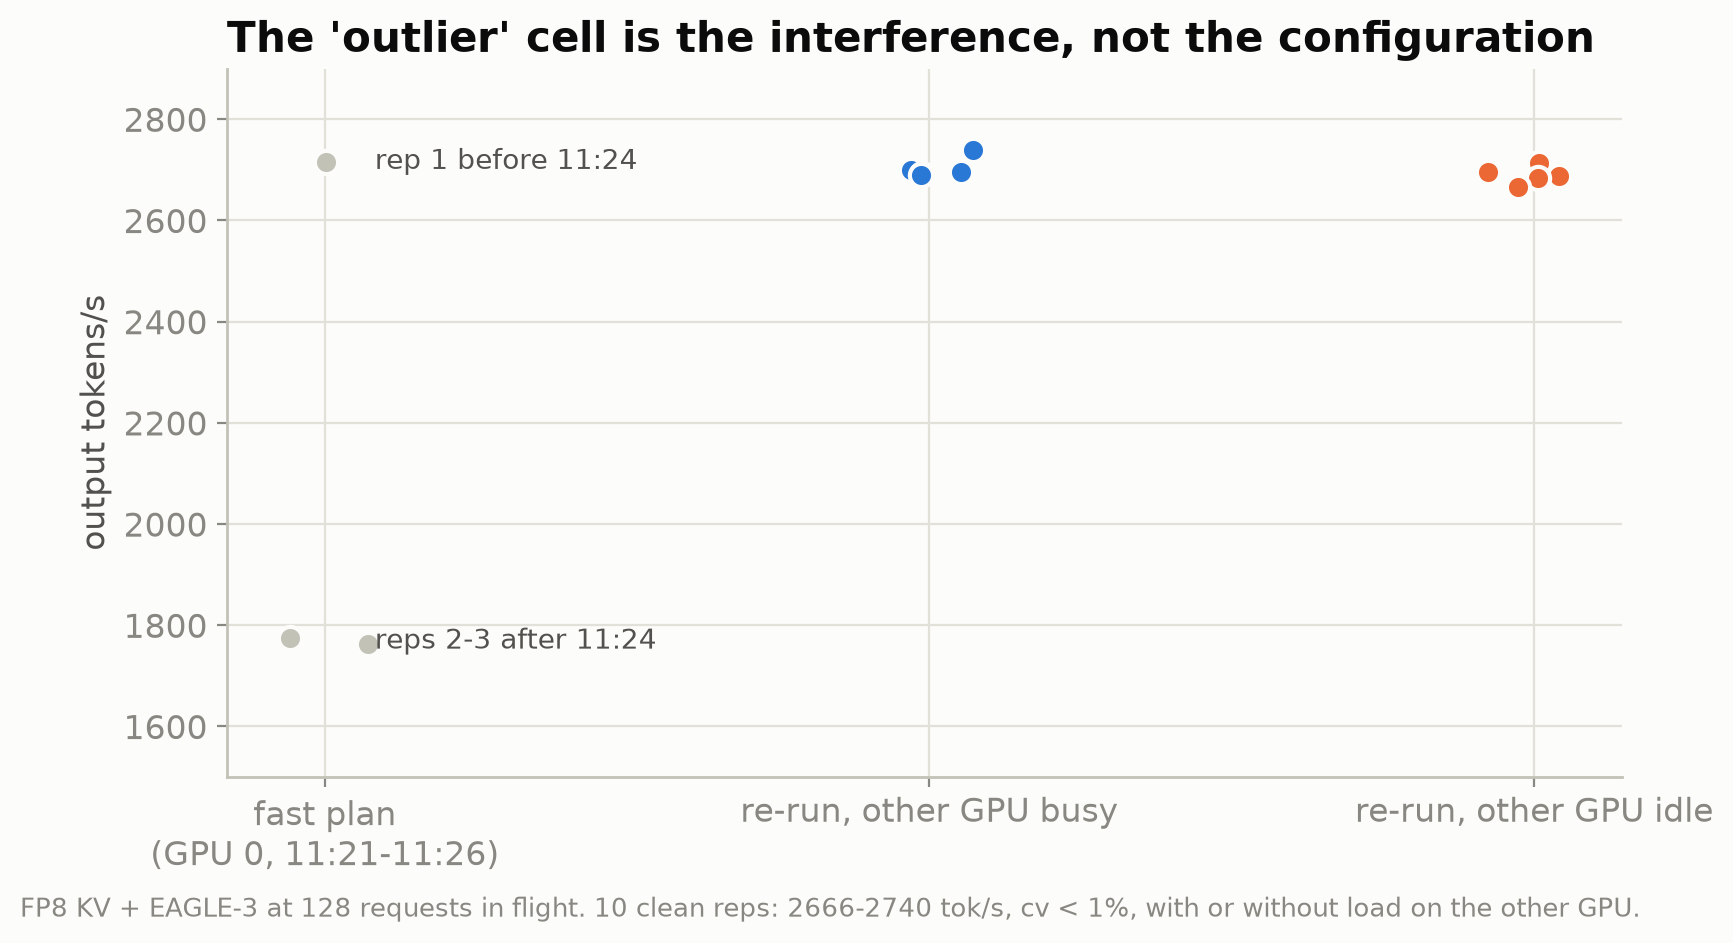
\includegraphics[width=0.49\linewidth]{figures/09_outlier_rerun.png}
\caption{Left: mean SM clock and power of Default at each workload. Right: the ``outlier'' cell, re-run 10 times
with the other GPU busy and idle.}
\end{figure}
\meas In all 18 profiler traces the GPU executed kernels 96--99\% of the time, dominated by cuBLAS GEMMs
(\texttt{nvjet\_*}); NVML reported the software power-cap throttle in all 126 investigation runs (mean power
394--400\,W of 400\,W), and Default's SM clock falls with load (1,493\,MHz at 2 in flight, 885\,MHz at 128). The
harness's first-order rule had labelled every final configuration ``per-step overhead''; the traces contradict it,
since there is almost no idle GPU time for CPU overhead to explain [C16]. \interp the binding constraint is
matrix-multiply work at power-capped clocks, so optimizations help in proportion to the GEMM work they remove (FP8,
spec, prefix), consistent with \S5.3. \meas Running two cells at once is sound: the cell that looked noisy in phase
1 was contamination, and re-run 5 times with the neighbouring GPU busy and 5 times idle it gave 2,690--2,740 and
2,666--2,713\,tok/s (CV $<$ 1\% each) [C17]. Checks \texttt{S5.7}.

\subsection{Conclusions, and tests not run}
\begin{takeaway}
\textbf{Supported by the evidence, for this workload:} (1) enable prefix caching whenever prompts repeat; it costs
nothing at 0\% reuse. (2) Enable EAGLE-3 for prompts up to $\sim$2--4k tokens, especially at low load; switch it off
beyond $\sim$4k. (3) FP8 weights are the most consistent single gain (1.22--1.34\x): pair them with \opt{spec}, but
not with FP8 KV where multi-step reasoning accuracy matters. (4) Tuning \texttt{max\_num\_seqs} is unnecessary
while the in-flight count stays below 256. (5) Predict combinations multiplicatively, not additively.
\textbf{Not run:} optimizations 6--7 on GPUs; joint extreme regimes; the 16 excluded cells; paired accuracy for
\opt{spec} combinations; real-traffic workloads; one unit test that needs the model tokenizer (skipped in the GPU-free
environment).
\end{takeaway}

% =====================================================================
\section{Milestone verification matrix}\label{sec:milestones}
% =====================================================================
Milestones are team-defined from Assignment 2 (\S D) and the progress report; no milestone or test IDs were issued
by the course for Project 24. ``Tests'' are the GPU-free commands anyone can run from a clean checkout: \texttt{pytest}
(\fp{tests/}, 69 tests: 68 passed, 1 skipped, 21 Nov), the dry pipeline, and \fp{evaluation/check_report_numbers.py}
(289/289 checks passed, 21 Nov), whose check ids are the test IDs below. \textbf{Changes:} no change was mentor-approved,
because no mentor feedback was received (\S\ref{sec:feedback}); the team-decided changes behind M4 and M6 are recorded in
ADR-012 and ADR-018.

{\small
\setlength{\tabcolsep}{3pt}
\begin{longtable}{@{}P{2.0cm}P{2.0cm}P{3.3cm}P{4.5cm}P{1.2cm}P{2.3cm}@{}}
\toprule
\rowcolor{tblhead}\hc{Milestone} & \hc{Test ID} & \hc{Expected} & \hc{Observed} & \hc{Status} & \hc{Evidence} \\
\midrule\endhead
M1 Scope \& design & -- & Problem, 7 optimizations, regimes, Value, run plan & Assignment 1, Assignment 2, progress
report & \pass & ADR-000, \fp{docs/progress/} \\
\rowcolor{rowgray} M2 Harness built & \texttt{pytest tests/}; dry pipeline & Unit tests, simulated end-to-end run, GPU
smoke test & 68/69 tests pass (1 needs the tokenizer); dry pipeline: 1,536 runs of the 7-optimization plan, 20
infeasible configs and 1 injected crash recorded, report written; smoke test 7/7 steps on 29 Oct & \pass &
\fp{tests/}, \fp{configs/profiles/dry.yaml}, \fp{SMOKE_TEST_REPORT.md} \\
M3 Baseline \& workload & \texttt{S5.1-cv}, \texttt{S2-base}, \texttt{S4-trace} & Default at 7 points, CV $\le$ 2\%;
Default truly all off; same trace per point & max Default CV 1.53\%; 45/45 Default runs verified off by the engine; 1
trace per point, 0 request errors in 510 runs & \pass & \fp{data/cells_combined_clean.csv}, ADR-003 \\
\rowcolor{rowgray} M4 Factorial measurement & \texttt{S4-runs}, \texttt{S5.2} & Planned design measured, $\ge$\,2
clean reps per cell & 384/384 runs ok; 112 clean phase-1 cells + 16 added; 16 lost to contamination; opts 6--7 not
run & \partl & ADR-012, \fp{data/cells_missing_after_cleaning.csv} \\
M5 Value \& table & \texttt{S5.1-*} & Value only when gates pass; Configuration \x\ Regime table & 0 latency, 86
accuracy failures; full table in App.\ A (generated from data) & \pass & App.\ A,
\fp{data/final_configs_by_policy.csv} \\
\rowcolor{rowgray} M6 Quality & \texttt{S5.6-*} & Accuracy vs.\ Default for every numeric setting & 8 settings
trimmed; 5 settings paired on full tasks; spec combinations not paired & \partl & ADR-018,
\fp{data/quality_paired_vs_default.csv} \\
M7 Attribution \& final config & \texttt{S5.3-*}, \texttt{S5.7} & Effects, interactions, Shapley, winner and binding
constraint per point & $R^2 \ge 0.9976$; Shapley exact at 3 points; 11/11 no-benefit cases explained; binding
constraint from 18 traces & \pass & \fp{data/clean_main_effects.csv}, \fp{data/clean_shapley.csv} \\
\rowcolor{rowgray} M8 Integrity & \texttt{S5.2}, \texttt{S5.7} & Contamination detected and removed; slots
independent; numbers reproducible & 71 runs flagged, 0 used; busy vs.\ idle CV $<$ 1\%; 289/289 checks & \pass &
ADR-017, ADR-020 \\
\bottomrule
\end{longtable}}

% =====================================================================
\section{Mentor feedback \& engineering evolution}\label{sec:feedback}
% =====================================================================
\textbf{Feedback closure.} No scored mentor feedback was received during the project, so there are no FB-IDs to close.

{\small
\begin{tabularx}{\linewidth}{@{}P{1.0cm}P{3.6cm}P{2.0cm}LP{2.6cm}@{}}
\toprule
\rowcolor{tblhead}\hc{FB-ID} & \hc{Mentor request} & \hc{Response / status} & \hc{Change / justification} & \hc{Evidence} \\
\midrule
-- & None received. & n/a & The progress report asked the mentor to confirm the GPU type and count, the latency target
and the quality tolerance; with no reply, the team fixed them itself (ADR-004, ADR-013, ADR-014). No change made after
the 9 October checkpoint has documented mentor approval; each is recorded in an ADR and listed below. &
\fp{docs/progress/} \\
\bottomrule
\end{tabularx}}

\medskip
\textbf{Engineering evolution.} The study was carried out as proposed in Assignment 2, with the changes below; each has
an ADR. The project first had
a 4\,\x\,RTX 6000 Ada (48\,GB) node; on 5 Nov it was downgraded to a Slurm node with two newer GPUs,
2\,\x\,H100 NVL (94\,GB). The largest change is the scope, decided on 2 Nov while the 4-GPU node was still the plan
(the full 7-optimization study was estimated at $\approx$\,95 node-hours, \fp{RUNBOOK.md} \S2) and kept after the
downgrade, which made it matter more. With seven optimizations the plan is 512 cells (128 at the centre + 6 \x\ 64), four times the 128 cells of five.
Parallelism also needs more than one GPU per cell, and in the harness every layout, including its ``off'' state, must
use all GPUs of a cell, so on the 2-GPU node cells could no longer run two at a time. At the measured 10.8
GPU-minutes per cell, the seven-factor factorial alone would need about 90\,h of node time (about twelve 8-hour jobs)
instead of 11.5\,h, close to the whole budget, before the extra sweeps for chunk size and layout. Chunked prefill
mainly targets tail latency rather than throughput, and on 2 GPUs only TP-2 versus two replicas would remain of the
four planned layouts. The time saved paid for phase 2, which found the contamination (ADR-012, ADR-016).

\begin{table}[H]
\small
\begin{tabularx}{\linewidth}{@{}P{3.1cm}P{4.2cm}LP{1.2cm}@{}}
\toprule
\rowcolor{tblhead}\hc{Item} & \hc{Assignment 2} & \hc{Final} & \hc{ADR} \\
\midrule
Quantized weights & W8A16 on an Ampere GPU (INT4 also considered) & FP8 W8A8 on FP8-capable GPUs & 007 \\
\rowcolor{rowgray} Speculation & EAGLE-style head or small draft model & EAGLE-3, 3 tokens; n-gram only for smoke tests
& 008 \\
Load generation & vLLM serving benchmark + async client & own closed-loop async client & 005 \\
\rowcolor{rowgray} Prompt sources & synthetic, ShareGPT, long documents & synthetic only (exact control) & 005 \\
Telemetry & DCGM / nvidia-smi, Nsight, Prometheus & NVML, Prometheus, torch profiler & 010 \\
\rowcolor{rowgray} Optimizations & all 7; 512 cells & 5 (chunked prefill and parallelism dropped); 128 cells & 012 \\
Hardware & one node, $k$ GPUs (Ampere assumed) & 4\,\x\,RTX 6000 Ada node, downgraded on 5 Nov to a 2\,\x\,H100 NVL
Slurm node (fewer, newer GPUs); one cell per GPU & 013, 014 \\
\rowcolor{rowgray} Phases & one factorial run + repeats of winners & factorial + anomaly investigation with paired
accuracy & 016, 018 \\
\bottomrule
\end{tabularx}
\end{table}

% =====================================================================
\section{Current state, limitations \& risks}
% =====================================================================
\begin{table}[H]
\small
{\rowcolors{2}{white}{rowgray}
\begin{tabularx}{\linewidth}{@{}>{\bfseries\raggedright\arraybackslash}p{1.5cm}L@{}}
\toprule
\rowcolor{tblhead}\hc{State} & \hc{Features} \\
\midrule
Working & Harness on vLLM 0.31.0 (resumable runs, hashed traces, telemetry, paired quality checks, analysis);
5-optimization factorial at 7 points (128 clean cells); all analyses of \S5; GPU-free unit tests, dry pipeline and
number checks. \\
Partial & Design coverage (16 cells missing); accuracy evidence for \opt{spec} combinations (policy B is an upper
bound); mechanism interpretations (F4--F6) consistent with telemetry but not proven by ablation; phase-2 CPU and
FLOP/byte telemetry unusable. \\
Missing & Optimizations 6--7 measured on GPUs; joint-extreme regimes; real-traffic workloads; a second model or GPU
type. \\
\bottomrule
\end{tabularx}}
\end{table}

\begin{table}[H]
\small
\begin{tabularx}{\linewidth}{@{}P{3.7cm}L@{}}
\toprule
\rowcolor{tblhead}\hc{Known defect / risk} & \hc{Impact and workaround} \\
\midrule
No GPU isolation on the shared node & A co-tenant slowed 18\% of phase-1 runs; the pre-flight VRAM check only runs at
job start (ADR-015). Workaround: re-run sample cells; compare device memory per run. \\
\rowcolor{rowgray} First-order binding rule & Labels every winner ``per-step overhead''; contradicted by traces (\S5.7). Use F9.\\
Technical debt & Run rows record \texttt{harness\_git = nogit}, so the exact harness revision of the 510 runs is not in
the data (ADR-011; the final tag is the reference revision). Phase-2 per-process CPU and FLOP/byte counters read 0
(fixed afterwards, not re-run; ADR-019). Optimization 7's multi-replica layouts ran only on the simulated engine. \\
\rowcolor{rowgray} Security & HumanEval's model-written code runs without a sandbox
in the measurement job on a shared node; future runs should isolate it. Dev-mode endpoints on per-job ports. No secrets or personal data.\\
Model provenance & Ungated mirror; checksums not compared with the official weights (ADR-002). \\
\rowcolor{rowgray} Validity limits & One model, one draft head, synthetic text, fixed 256-token outputs, closed-loop load, power-capped
GPU, 2--3 reps, one greedy accuracy run per setting. \\
\bottomrule
\end{tabularx}
\end{table}

% =====================================================================
\section{Way forward}
% =====================================================================
The next steps, in priority order:

\begin{enumerate}
\item \textbf{Paired accuracy for the FP8 + speculation settings.} Run the paired quality test on quant+spec, kvq+spec
and all three together, so we know whether the faster configurations are usable. \emph{Start from:}
\fp{configs/profiles/investigate.yaml} (\texttt{quality.settings}) and \fp{harness/analysis/investigate.py}.
\emph{Depends on:} one GPU for a few hours, in a sandboxed job (HumanEval runs model-written code). \emph{Done when:}
we have accuracy results and per-question answers for each setting, with a paired 95\% interval on GSM8K, HumanEval
and MMLU, so the policy-B speedups (up to 3.30\x) are either confirmed or withdrawn.
\item \textbf{Prompt-length sweep for speculative decoding.} Run finer steps between 2k and 8k tokens to pin down where
EAGLE-3 stops helping. \emph{Start from:} the \texttt{spec\_long\_context} investigation in \fp{investigate.yaml} and
\fp{data/spec_vs_context.csv}. \emph{Depends on:} one GPU for a few hours. \emph{Done when:} we have speedup,
acceptance and telemetry at each length, and the length at which EAGLE-3's speedup falls to 1.00\x\ is located to
within 512 tokens.
\item \textbf{Chunked prefill and parallelism.} Measure both on a node with at least four GPUs. \emph{Start from:} bits
6--7 in \fp{harness/engine/vllm_flags.py} and \fp{configs/profiles/full.yaml}. \emph{Depends on:} about 25 node-hours;
\emph{blocker:} the current node has only two GPUs. \emph{Done when:} we have throughput, latency and telemetry for
each, and can explain what they do: their main effects at the centre with $R^2 \ge 0.99$, and non-zero CPU and
FLOP/byte telemetry.
\item \textbf{Real-traffic workload.} Replay real multi-turn prompts instead of synthetic ones. \emph{Start from:}
\texttt{workload.source} in \fp{configs/experiment.yaml}. \emph{Depends on:} a dataset with a suitable licence;
prompt lengths are no longer under our control. \emph{Done when:} we have results and telemetry on real traffic, and
can compare them with the synthetic runs: EAGLE-3 acceptance and prefix hit rate are reported, and every main effect
is within 10\% of the synthetic one or the difference is explained.
\end{enumerate}

% =====================================================================
\section{Contributions, AI use \& attribution}
% =====================================================================
\begin{table}[H]
\small
{\rowcolors{2}{white}{rowgray}
\begin{tabularx}{\linewidth}{@{}P{2.6cm}LP{4.6cm}@{}}
\toprule
\rowcolor{tblhead}\hc{Member} & \hc{Meaningful areas / modules} & \hc{PR / commit evidence} \\
\midrule
Panshul Jindal & Initial project planning, with Mohd Shozab (scope, optimizations, regimes, run plan). Final
review and writing of this report and the presentation, from Shozab's initial drafts: course-guide compliance
(\S6 test IDs, \S7 feedback closure), corrections of overstated claims in the report, slides and script, an added
number check (\texttt{S5.2}), the repository restructure to the handover layout, and the readable edition
of the report. & Commits
\href{https://github.com/Panshul-Jindal/SpeedingUpLLMInference/commit/4878541503bf0dc5d6a3b0e941c37efaa63cb6ce}{\texttt{4878541}} (restructure),
\href{https://github.com/Panshul-Jindal/SpeedingUpLLMInference/commit/ae8922bbbcfabfbe7f4fbdc927f4e35ada2d742a}{\texttt{ae8922b}} (review fixes),
\href{https://github.com/Panshul-Jindal/SpeedingUpLLMInference/commit/77d9ee8}{\texttt{77d9ee8}} (\S10),
\href{https://github.com/Panshul-Jindal/SpeedingUpLLMInference/commit/e1c43c5}{\texttt{e1c43c5}} (readable edition) \\
Mohd Shozab & Initial project planning, with Panshul Jindal. Everything else: the measurement harness
(\fp{harness/}: configuration, design, vLLM launcher, workload, load driver, telemetry, quality checker, analysis,
orchestrator), its 69 unit tests and the Slurm/cluster scripts; running phase 1 and phase 2 on the H100 node;
contamination detection, data cleaning and the report pack; the number-check and figure scripts; and the initial
drafts of the report, ADRs and presentation. & Original harness history (commits \texttt{6ebfa6d} to
\texttt{c42acca}, cited in the ADRs; not yet imported into this repository); import commit
\href{https://github.com/Panshul-Jindal/SpeedingUpLLMInference/commit/4300642b7d3810d7eac72616de71af8cc8a158a4}{\texttt{4300642}};
\fp{docs/progress/2026-10-29_harness_handoff.pdf} \\
\bottomrule
\end{tabularx}}
\end{table}

\textbf{AI-assisted work.} \emph{Report generation (Claude-assisted).} This report, the ADR write-up,
\fp{evaluation/check_report_numbers.py}, \fp{evaluation/make_report_figures.py} (figures 10--12 and Appendix A) were
drafted with Claude (Anthropic); the final review, the repository restructure and the readable edition were done with
Claude Code. \emph{How it was checked:} every number in the text is recomputed from the committed CSVs by the check
script (289/289 pass), which found two errors in earlier drafts (claim C2 and one rounding), both corrected; figures
10--12 and Appendix A are generated, not typed; the unit tests were re-run; the team reviewed the text against the
code and data.

\textbf{Third-party assets.} Reused software, model weights and datasets are listed with versions and licences in
\S2; weights and datasets are downloaded at run time and are not redistributed. Figures and data are the team's own
measurements.

% =====================================================================
% References
% =====================================================================
\begingroup
\small
\renewcommand{\section}[2]{\vspace{1ex}\noindent{\sffamily\large\bfseries\color{accent}References}\par\vspace{0.3ex}}
\begin{thebibliography}{99}
\setlength{\itemsep}{1pt}
\bibitem{vllm} W.~Kwon et al. Efficient Memory Management for Large Language Model Serving with PagedAttention. SOSP 2023.
\bibitem{sglang} L.~Zheng et al. SGLang: Efficient Execution of Structured Language Model Programs. NeurIPS 2024.
\bibitem{sarathi} A.~Agrawal et al. Taming Throughput-Latency Tradeoff in LLM Inference with Sarathi-Serve. OSDI 2024.
\bibitem{orca} G.-I.~Yu et al. Orca: A Distributed Serving System for Transformer-Based Generative Models. OSDI 2022.
\bibitem{leviathan} Y.~Leviathan, M.~Kalman, Y.~Matias. Fast Inference from Transformers via Speculative Decoding. ICML 2023.
\bibitem{chen} C.~Chen et al. Accelerating Large Language Model Decoding with Speculative Sampling. arXiv:2302.01318, 2023.
\bibitem{eagle} Y.~Li, F.~Wei, C.~Zhang, H.~Zhang. EAGLE: Speculative Sampling Requires Rethinking Feature Uncertainty. ICML 2024.
\bibitem{eagle3} Y.~Li et al. EAGLE-3: Scaling up Inference Acceleration of Large Language Models via Training-Time Test. arXiv:2503.01840, 2025.
\bibitem{fp8} P.~Micikevicius et al. FP8 Formats for Deep Learning. arXiv:2209.05433, 2022.
\bibitem{kivi} Z.~Liu et al. KIVI: A Tuning-Free Asymmetric 2bit Quantization for KV Cache. ICML 2024.
\bibitem{cacheblend} J.~Yao et al. CacheBlend: Fast Large Language Model Serving for RAG with Cached Knowledge Fusion. EuroSys 2025.
\bibitem{distserve} Y.~Zhong et al. DistServe: Disaggregating Prefill and Decoding for Goodput-optimized Large Language Model Serving. OSDI 2024.
\bibitem{pope} R.~Pope et al. Efficiently Scaling Transformer Inference. MLSys 2023.
\bibitem{gqa} J.~Ainslie et al. GQA: Training Generalized Multi-Query Transformer Models from Multi-Head Checkpoints. EMNLP 2023.
\bibitem{llama3} Llama Team, AI @ Meta. The Llama 3 Herd of Models. arXiv:2407.21783, 2024.
\bibitem{gsm8k} K.~Cobbe et al. Training Verifiers to Solve Math Word Problems. arXiv:2110.14168, 2021.
\bibitem{humaneval} M.~Chen et al. Evaluating Large Language Models Trained on Code. arXiv:2107.03374, 2021.
\bibitem{mmlu} D.~Hendrycks et al. Measuring Massive Multitask Language Understanding. ICLR 2021.
\bibitem{lmeval} EleutherAI. lm-evaluation-harness, v0.4.13. \url{https://github.com/EleutherAI/lm-evaluation-harness}
\bibitem{box} G.~E.~P.~Box, J.~S.~Hunter, W.~G.~Hunter. Statistics for Experimenters, 2nd ed. Wiley, 2005.
\bibitem{mcnemar} Q.~McNemar. Note on the Sampling Error of the Difference Between Correlated Proportions or Percentages. Psychometrika 12(2), 1947.
\bibitem{shapley} L.~S.~Shapley. A Value for n-Person Games. Contributions to the Theory of Games II, Princeton, 1953.
\bibitem{roofline} S.~Williams, A.~Waterman, D.~Patterson. Roofline: An Insightful Visual Performance Model for Multicore Architectures. CACM 52(4), 2009.
\bibitem{amdahl} G.~M.~Amdahl. Validity of the Single Processor Approach to Achieving Large Scale Computing Capabilities. AFIPS 1967.
\bibitem{awq} J.~Lin et al. AWQ: Activation-aware Weight Quantization for LLM Compression and Acceleration. MLSys 2024.
\end{thebibliography}
\endgroup

% =====================================================================
% Appendices
% =====================================================================
\clearpage
\appendix
\renewcommand{\thesection}{\Alph{section}}
\section{Configurations \x\ regimes (problem-statement table)}
Throughput speedup over Default for every configuration at every workload point, generated from
\fp{data/cells_combined_clean.csv} by \fp{evaluation/make_report_figures.py}. Value equals this speedup when all gates
pass; $\dagger$ = failed the original accuracy gate (policy A), so Value is 1.00. No cell failed a latency gate.
``--'' = not in the half-fraction design, or excluded after contamination. Bits: quant kvq spec prefix batch;
shaded rows contain FP8 KV.

{\footnotesize
\setlength{\tabcolsep}{3pt}
\renewcommand{\arraystretch}{1.02}
\begin{longtable}{@{}lc*{7}{r}@{}}
\toprule
\rowcolor{tblhead}\hc{Configuration} & \hc{Bits} & \hc{Centre} & \hc{Short} & \hc{Long} & \hc{Low conc.} & \hc{High conc.} & \hc{0\% reuse} & \hc{90\% reuse} \\
\midrule\endhead
\inputtable{appendix_config_x_regime.tex}
\bottomrule
\end{longtable}}

\section{Evidence index}
\begin{table}[H]
\small
{\rowcolors{2}{white}{rowgray}
\begin{tabularx}{\linewidth}{@{}LP{8.6cm}@{}}
\toprule
\rowcolor{tblhead}\hc{Evidence} & \hc{Location} \\
\midrule
Every phase-1 run (384, with contamination flag) & \fp{evaluation/report_pack/data/runs_fast_plan_all.csv} \\
Every phase-2 run (126, deep telemetry) & \fp{evaluation/report_pack/data/runs_investigation.csv} \\
Cleaned runs (363) and cells (128) & \fp{data/runs_combined_clean.csv}, \fp{data/cells_combined_clean.csv} \\
Findings, claims, per-configuration notes & \fp{FINDINGS.md}, \fp{CLAIMS.csv}, \fp{CONFIG_NOTES.md} \\
Methodology, limitations, data dictionary & \fp{METHODOLOGY.md}, \fp{LIMITATIONS.md}, \fp{DATA_DICTIONARY.md} \\
Figures 01--12 & \fp{evaluation/report_pack/figures/} \\
Number checks (289) and generated figures & \fp{evaluation/check_report_numbers.py},
\fp{evaluation/make_report_figures.py} \\
Unit tests (69) and dry run & \fp{tests/}, \fp{configs/profiles/dry.yaml} \\
Architecture Decision Records & \fp{docs/Architecture_Decision_Records.md} (ADR-000 to ADR-020) \\
Build spec, smoke test, runbook & \fp{docs/build_spec.md}, \fp{SMOKE_TEST_REPORT.md}, \fp{RUNBOOK.md} \\
Experiment profiles & \fp{configs/profiles/fast.yaml}, \fp{configs/profiles/investigate.yaml} \\
\bottomrule
\end{tabularx}}
\end{table}

\end{document}
